\documentclass{article}
\usepackage[T1]{fontenc}
\usepackage[hyphens]{url}
\usepackage{algorithm}
\usepackage{algpseudocode}
\usepackage{amsbsy}
\usepackage{amsmath}
\usepackage{amssymb}
\usepackage{amsthm}
\usepackage{authblk}
\usepackage{caption}
\usepackage{datetime}
\usepackage{fancyvrb}
\usepackage{framed}
\usepackage{fixltx2e}
\usepackage{graphicx}
\usepackage{listings}
\usepackage{manfnt}
\usepackage{marvosym}
\usepackage{mathrsfs}
\usepackage{mathtools}
\usepackage{multicol}
\usepackage{nicefrac}
\usepackage{setspace}
\usepackage{stmaryrd}
\usepackage{textcomp}
\usepackage{tikz}
\usepackage{upquote}
\usepackage{xcolor}

\DeclareGraphicsExtensions{.png,.jpg}

\theoremstyle{plain}
\newtheorem{cor}{Corollary}
\newtheorem{defin}{Definition}
\newtheorem{lem}{Lemma}
\newtheorem{notation}{Notation}
\newtheorem{pro}{Proposition}
\newtheorem{rem}{Remark}
\newtheorem{thm}{Theorem}

\newtheorem{prob}{Problem}
\let\oldprob\prob
\renewcommand{\prob}{\oldprob\normalfont}

%\theoremstyle{definition}
\newtheorem{exa}{Example}

\newcommand{\codefont}[1]{{\fontshape{n}\texttt{#1}}}

\newcommand{\backtick}{$\hspace{4pt}\grave{ }\hspace{2pt}$}
\newcommand{\norm}[1]{\lVert#1\rVert}
\newcommand*\circled[1]{\tikz[baseline=(char.base)]{
            \node[shape=circle,draw,inner sep=1pt] (char) {#1};}}
\newcommand{\boxd}[1]{\fbox{
  \begin{minipage}{6.5in}#1\end{minipage}}}
\DeclareMathOperator{\Var}{Var}
\DeclareMathOperator{\Arg}{Arg}
\DeclareMathOperator{\fix}{fix}
\DeclareMathOperator{\Fix}{Fix}
\DeclareMathOperator{\aut}{aut}
\DeclareMathOperator{\Id}{Id}

\usetikzlibrary{automata,positioning}

\DeclareCaptionFormat{algor}{%
  \hrulefill\par\offinterlineskip\vskip1pt%
    \textbf{#1#2}#3\offinterlineskip\hrulefill}
\DeclareCaptionStyle{algori}{singlelinecheck=off,format=algor,labelsep=space}

\newenvironment{snippet}{\VerbatimEnvironment\fontfamily{ppl}
\selectfont
\begin{Verbatim}}{\end{Verbatim}}

\newenvironment{sol}{%
  \noindent\textbf{Solution: }}{}

\newenvironment{mathematica}{%
  \def\FrameCommand{\fboxsep=\FrameSep \fcolorbox{black}{gray}}%
  \color{black}\MakeFramed {\FrameRestore}\textbf{Mathematica note: }}%
 {\endMakeFramed}

% http://stackoverflow.com/a/1670572/371334
\newenvironment{changemargin}[2]{%
\begin{list}{}{%
\setlength{\topsep}{0pt}%
\setlength{\leftmargin}{#1}%
\setlength{\rightmargin}{#2}%
\setlength{\listparindent}{\parindent}%
\setlength{\itemindent}{\parindent}%
\setlength{\parsep}{\parskip}%
}%
\item[]}{\end{list}}

% New definition of square root:
% it renames \sqrt as \oldsqrt
\let\oldsqrt\sqrt
% it defines the new \sqrt in terms of the old one
\def\sqrt{\mathpalette\DHLhksqrt}
\def\DHLhksqrt#1#2{%
\setbox0=\hbox{$#1\oldsqrt{#2\,}$}\dimen0=\ht0
\advance\dimen0-0.2\ht0
\setbox2=\hbox{\vrule height\ht0 depth -\dimen0}%
{\box0\lower0.4pt\box2}}

% http://tex.stackexchange.com/a/33998/8865
\newcommand\BrText[2]{%
  \par\smallskip
   \noindent\makebox[\textwidth][r]{$\text{#1}\hspace{9pt}
    \begin{minipage}{\textwidth}
    #2
    \end{minipage}
  \nulldelimiterspace=0pt$}\par\smallskip
}


\begin{document}
\title{Genfunlib: A Mathematica package for combinatorial power series}
\author{Andrew MacFie}
\date{2014}
\maketitle


\section*{Abstract}
Generating functions (i.e.\ power series) have applications throughout
enumerative and analytic combinatorics.
In this document we present Genfunlib, a new Mathematica package containing a
selection of implementations of symbolic methods related to generating
functions.
With Genfunlib one can find the generating functions for regular languages,
compute the initial terms of a generating function, convert between
generating function equations and recurrences, and find asymptotics.
This document gives mathematical background, extensive documentation for
Genfunlib, and tutorials.


\tableofcontents





\section{Introduction}

\noindent
This document is on Genfunlib, a package for the Mathematica computer algebra
system, which was written by the author of this document.
The goal of Genfunlib is to provide commands for obtaining and using generating
functions to solve combinatorial problems.
The package is available for download at\\
\url{https://github.com/amacfie/Genfunlib}

% contributions
Genfunlib consists of implementations of a number of well--known procedures not
currently available in Mathematica or any third--party Mathematica package.
Genfunlib includes comprehensive finite automata functionality that allows
the user to convert between automata and regular expressions, and perform
standard operations such as union, intersection, and reversal.
Generating functions that count the number of words in a given regular language
can be computed.
These generating functions can be useful for counting problems that involve
regular languages such as pattern avoidance in words.
Genfunlib uses known methods to produce asymptotic information about a counting
sequence given its generating function.
From a power series equation, Genfunlib can compute the initial terms of the
solution series.
Genfunlib improves on Mathematica's built--in capabilities for converting
between recurrence relations and power series equations.
The symbolic method for obtaining generating functions from constructible
combinatorial classes is also implemented in Genfunlib.

The contents of this document are as follows.
In Section \ref{sec:aofa}, we give an overview of enumerative combinatorics,
generating functions, and their applications to analysis of algorithms.
Thanks to this section, the mathematical content of this document is fairly
self--contained.
Section \ref{sec:mma} is a brief overview of Mathematica programming to allow
readers to better understand the code in this document.
Section \ref{sec:guide} goes through each of Genfunlib's commands and explains
how to use them, what they do and, where educative, how they do it.
It is divided into subsections that cover all the commands related to one
mathematical topic.
This section can be considered to be both user and developer documentation.
Boxes labeled ``Mathematica note'' can be ignored by readers unfamiliar with
Mathematica.
In Section \ref{sec:action} we present a number of relatively elementary
combinatorial problems, and solutions
that make use of Genfunlib and Mathematica.
In the solutions, we attempt to give a sense of the range of Genfunlib's
functionality and try to minimize the number of operations performed
``by hand''.
The problems in Section \ref{sec:contest} come from high school mathematics
contests, or contest preparation material.
Finally, in Section \ref{sec:conc} we conclude by offering possible paths
for further work.

Naturally, Genfunlib does not implement all known algorithms that one may want
to use with generating functions.
Areas for expansion and improvement are discussed as they are relevant at
various points in the body of the document.
Further, there are tests and operations on power series for which no
algorithm has been found, e.g.\ whether a given univariate rational
function has only positive coefficients
\cite{kauers2007computer}.


\section{Mathematics for the analysis of algorithms} \label{sec:aofa}
\begin{quote}
  \emph{In theoretical computer science, the greatest
innovation is the realisation that algorithms are mathematical objects, and can
be rigorously analysed in terms of their consumption of scarce resources,
including space, time, and randomness.}
\end{quote}
\hfill -- Jeffrey Shallit, 2006 \cite{shal}\\

\noindent
Given a computer program, one may desire to know how long it will take to run in
absolute terms, that is, in physical units of time.
Indeed ultimately, such concrete predictions are always the end goal,
and engineering methods involving statistics, simulation, and detailed
knowledge of particular computing environments are certainly used
(when rigorous this is known as the \emph{experimental analysis of
algorithms}).
However, given the complexity of actual computers, a more abstract problem is
taken to be the typical one in the field of computer science called
\emph{analysis of algorithms}.

First, instead of executable computer programs, the objects of study are
\emph{algorithms} \cite{guralg},
generally given at a level of abstraction where pseudocode
is sufficient.
The physical running time of an algorithm is not defined, but the number
of steps it takes is.
It is assumed that the number of steps taken by an algorithm gives information
related to actual running time of computer implementations.
From now on, the ``running time'' of an algorithm means the number of steps
it takes.

Second, because algorithms are abstract objects and do not run on computers,
the goal is not to predict absolute timings, but to compare algorithms
with each other.
Let \( T(A, i) \) be the running time of an algorithm \( A \) on an input
\( i \).
Let \( I(n) \) be the set of inputs with size \( n \).
We can represent the running time of \( A \) with respect to a probability
mass function \( f_n : I(n) \rightarrow [0, 1] \) by the sequence
\[
  (T_A(n)), \text{ where } T_A(n) = \sum_{ i \in I(n) } T(A, i) f_n(i).
\]
That is, \( T_A(n) \) is the expected running time of \( A \) according to the
probability distribution defined by \(f_n\).
The most common distribution is ``worst--case'', which assigns probability
\( 1 \) to an input in \( I(n) \) on which the running time of \( A \) is
maximal.
Another common distribution used is ``average--case'', where
\[
  f_n(i) = 1 / |I(n)|,
\]
for all \( i \).
More nuanced analysis has been done beyond these two distributions,
notably smoothed analysis and analysis using the Solomonoff--Levin measure
\cite{livit}.

Once the distribution has been chosen, for two algorithms \(A\) and \(B\)
computing the same
function, we have the two sequences \( (T_A(n)) \) and \( (T_B(n)) \).
Obviously, if \( T_A(n) \geq T_B(n) \) for all \(n\), it is easy to compare
\(A\) and \(B\), but this ordering is not always enough.
Instead, analysis of algorithms uses \emph{asymptotics}:
relations are established between \( T_A(n) \) and \( T_B(n) \) as \( n \)
approaches infinity.
Now, instead of directly comparing \(T_A(n) \) to \(T_X(n) \) for each \( X \),
we can, analogously to  the ``interlingua'' approach to machine translation
\cite{jurafsky2000speech},
find a relation between \(T_A(n) \) and a simple standard sequence, after
which, to compare algorithms we need only compare simple standard sequences,
which is easy.

\begin{defin}[Asymptotic notation]
  As \( n \rightarrow \infty \),
  \begin{itemize}
    \item \( f(n) = O(g(n)) \) means
      \( \exists c > 0, N > 0 : \forall n, \ n > N \implies f(n) < c g(n) \),
    \item \( f(n) = \Omega(g(n)) \) means \( g(n) = O(f(n)) \),
    \item \( f(n) = \Theta(g(n)) \) means \( f(n) = O(g(n)) \) and
      \( g(n) = O(f(n)) \),
    \item \( f(n) = o(g(n)) \) means
      \( \lim_{n \rightarrow \infty} \frac{g(n)}{f(n)} = \infty \),
    \item \( f(n) \sim g(n) \) means
      \( \lim_{n \rightarrow \infty} \frac{g(n)}{f(n)} = 1 \), and
    \item \( f(n) = \omega(g(n)) \) means
      \( \lim_{n \rightarrow \infty} \frac{g(n)}{f(n)} = 0 \).
  \end{itemize}
\end{defin}

\begin{exa}

  Suppose \( T_A(n) =  \sum_{k=1}^n \frac{n}{k} \),
  \( T_B(n) = 2^n \), and
  \( T_C(n) = \frac{1}{n+1} \binom{2n}{n} \).
  Then we have, as \( n \rightarrow \infty, \)
  \begin{align*}
    T_A(n) &= \Theta(n \log(n)), \\
    T_B(n) &= \Theta(2^n), \\
    T_C(n) &= \Theta \left( \frac{4^n}{n^{3/2}} \right).
  \end{align*}
  By comparing \(  n \log(n), 2^n, \) and \( \frac{4^n}{n^{3/2} } \),
  we see \( T_A(n) = o(T_B(n)) \) and \( T_B(n) = o(T_C(n)), \) as \(n
  \rightarrow \infty. \)

\end{exa}

Asymptotics in this setting are perhaps surprisingly useful.
The obvious objection to their use is that, for example, even though
\( (1 + \exp(-10^{10}))^n \) is in every asymptotic sense greater than
\( n^{100} \), the former is in every practical sense less than the latter.
It is simply an observed fact that asymptotic statements are usually
practically relevant, even though so much information is lost.

Thus, we see that the prototypical methodology in analysis of algorithms is
the (incomputable in general) passage from algorithms to running
time sequences to asymptotic expressions.
(As always in mathematics, more abstract problems may be solved in analysis
of algorithms which support this methodology indirectly.)
This progression can be broken down into its two stages.

Obtaining exact running time sequences is closely related to the field of
mathematics called enumerative combinatorics, a.k.a.\ counting.
For example, let \(S_n\) be the highest--cardinality set of states that an
algorithm \(A\) enters on an input of size \(n\).
Then \( |S_n| \) is the worst--case running time of \( A \) on inputs of size
\( n \).
Counting sets such as \(S_n\) is precisely the field of enumerative
combinatorics.
According to Wilf \cite{wilf}, when an algorithm is found that takes
\( n \) and returns \( |S_n| \) and runs in at
most exponential time, the combinatorial counting problem associated with
the sets \( S_n \) has been solved.
To obtain these cardinality algorithms, a set of counting
strategies/techniques is used, including the principle of inclusion--exclusion,
recurrences, refinements, decompositions, and P\'olya theory.

Instead of passing directly from a set to its cardinality, in enumerative
combinatorics, establishing a bijection between two sets is a very common
goal.
If something has been proved about the cardinality of a set \( S_1 \), which
is shown to be in bijection with \(S_2\), the same result applies to \(S_2\).

Problems in enumerative combinatorics may come from places
other than analysis of algorithms, such as combinatorial number theory,
algebra, and graph theory.

Given a sequence \( (f_n), \) we define the \emph{ordinary generating function}
of \( (f_n) \) to be
\[
  F(z) = \sum_{n \geq 0} f_n z^n,
\]
and we define the \emph{exponential generating function} of \( (f_n) \) to be
\[
  \hat{F}(z) = \sum_{n \geq 0} f_n \frac{z^n}{n!}.
\]
It turns out that these power series representations can be very useful for
solving combinatorial problems, and especially useful for obtaining an
asymptotic estimate of a sequence.

We define two common classes of power series.
A power series \( f(z) \in \mathbb{Q}[[z]] \) is \emph{algebraic} iff there
exist \( p_0(z), \dots, p_j(z) \in \mathbb{Q}[z] \) such that
\[
  \sum_{k=0}^j p_k(z) f(z)^k = 0.
\]
A power series \( f(z) \in \mathbb{Q}[[z]] \) is \emph{holonomic} iff there
exist \( p_0(z), \dots, p_j(z) \in \mathbb{Q}[z] \) such that
\[
  \sum_{k=0}^j p_k(z) f(z)^{(k)} = 0,
\]
where \( f(z)^{(k)} \) is the \(k\)th formal derivative of \( f(z). \)
Algebraic power series are holonomic \cite{ec2}.





\section{A few notes on Mathematica} \label{sec:mma}

In order to fully understand all of the Mathematica code used in this document,
the reader would have to be quite familiar with the Mathematica programming
language.
Ruskeep{\"a}{\"a}'s book \cite{mmabook} is ample preparation, for example.
However, readers who are not familiar with Mathematica should still be able to
follow the important ideas, and this section provides some essential
Mathematica information to help in this regard.

The Mathematica code in this document is shown as it appears in an interactive
session: There are input lines, which are typed in by the user after the
prompt \codefont{In[k]:= }, and output
lines, which Mathematica returns.
Input lines that end in a semicolon do not produce an output line.
Here is a basic example:
\begin{snippet}
In[1]:= 2 + 2

Out[1]= 4

In[2]:= 3 + 3

Out[2]= 6
\end{snippet}
Every input line is numbered and its output line has the same number.

The character \codefont{\%} stands for the expression in the previous output
line.

\begin{snippet}
In[3]:= 4 - 2

Out[3]= 2

In[4]:= % - 2

Out[4]= 0
\end{snippet}

In Mathematica, functions take their arguments in square brackets.
\begin{snippet}
In[5]:= Sin[Pi]

Out[5]= 0
\end{snippet}
To write an anonymous function, write the value in terms of
the argument \codefont{\#}, and place an \codefont{\&} at the end.
In the next snippet, we define a function \codefont{f} that squares its
argument.
\begin{snippet}
In[6]:= f = #^2 &;

In[7]:= f[4]

Out[7]= 16
\end{snippet}

Some of Mathematica's built--in functions use assumptions to control their
behavior.
They work like this:
\begin{snippet}
In[8]:= FullSimplify[(-1)^(2a)]

Out[8]= (-1)^(2a)

In[9]:= FullSimplify[(-1)^(2a), Assumptions ->
    Element[a, Integers]]

Out[9]= 1
\end{snippet}
In \codefont{In[9]} we pass an \codefont{Assumptions} option to the algebraic
simplifier function \codefont{FullSimplify} that says \codefont{a} can be
assumed to be an integer.
Alternatively, assumptions can be specified by setting the global
\codefont{\$Assumptions} variable:
\begin{snippet}
In[10]:= $Assumptions = Element[a, Integers];

In[11]:= FullSimplify[(-1)^(2a)]

Out[11]:= 1
\end{snippet}

Lists in Mathematica are made with braces and commas:
\begin{snippet}
In[12]:= list = {5, 4, 3, 2, 1, 0};

In[13]:= Length[list]

Out[13]= 6
\end{snippet}
Mathematica lists can contain anything:
\begin{snippet}
In[14]:= l = {5, "this is a string", {"string in a nested list!",
    True, symbol}};
\end{snippet}

It is perfectly fine for a function to not evaluate:
\begin{snippet}
In[15]:= Sin[2]

Out[15]= Sin[2]
\end{snippet}
If we want the numerical value of \( \sin(2), \) for example, we pass it to the
\codefont{N} function:
\begin{snippet}
In[16]:= N[Sin[2]]

Out[16]= 0.909297
\end{snippet}

Mathematica has a huge number of built--in functions.
To learn about a built--in function, simply search the online documentation
\cite{mmadoc}.

\section{Guide to Genfunlib} \label{sec:guide}

% math discussion, user docs, dev docs

\subsection{Power series and their coefficients}

Converting between power series and their sequences of coefficients is a basic
operation in computer algebra.
In general, power series are represented by equations that they satisfy, which
may be differential equations.
This includes equations implied by ``closed--form'' expressions.
Analogously, sequences may be given by recurrence relations or closed--form
expressions.

It is tempting to say that when performing the conversion between power series
and coefficient sequences,
closed--form power series equations should become
closed--form expressions for coefficients, and nontrivial power series equations
should become recurrence relations.
However, while it generally can, why \emph{should} this aspect of the structure
of an equation be preserved?
Why not transform \[ F(z) = \frac{1}{1 - 2z} \] to
\[ f_n = 2 f_{n-1}, \qquad f_0 = 1 \qquad \text{instead of} \qquad f_n = 2^n?\]
Indeed, if one wants a recurrence relation for computing initial terms,
for computational efficiency reasons it is preferrable to have a
recurrence relation that includes a finite set of lower-index terms,
as opposed to one that uses the full-history of the sequence.
Thus, unless the form that the result should be in is explicitly stated, there
are many ways the translation can be performed \cite{simpl}.

Mathematica 9 includes some functionality for converting between power series
and their coefficient sequences;
Genfunlib extends this functionality by increasing the set of power series
equations/recurrence relations on which the transformation can be applied.

\begin{mathematica}
  In computer algebra, representing a power series by an equation it satisfies
  is useful because of the level of generality it affords.
  Mathematica has support for two kinds of power series equation objects
  that can be used with \codefont{Series} and \codefont{SeriesCoefficient}.

  Solutions to linear differential equations are represented as
  \codefont{DifferentialRoot} objects:

  \begin{snippet}
In[17]:= FullSimplify[
    SeriesCoefficient[
    DifferentialRoot[Function[{y, x}, {y'[x] == y[x], y[0] == 1}
    ]][x], {x, 0, n}],
    Assumptions :> Element[n, Integers] && n >= 0]

Out[17]= 1/n!
  \end{snippet}

  Solutions to algebraic equations are represented as \codefont{Root} objects:

  \begin{snippet}
In[18]:= Series[Root[#^5+a #+1&,1],{a,0,5}]

Out[18]= -1+a/5+a^2/25+a^3/125-(21 a^5)/15625+O[a]^6
  \end{snippet}
\end{mathematica}

Genfunlib overrides the \codefont{SeriesCoefficient} command for extracting
the coefficients of a power series.

Using Mathematica's built--in \codefont{SeriesCoefficient} we can compute the
coefficients of explicit power series like \(\exp(z)\).

\begin{snippet}
In[19]:= $Assumptions=(n>=0);

In[20]:= SeriesCoefficient[Exp[z],{z,0,n}]

Out[20]= 1/n!
\end{snippet}

Genfunlib adds the ability to work with \emph{symbolic} power series, as in the
following example.

\begin{snippet}
In[21]:= $FullAnalytic=True;

In[22]:= SeriesCoefficient[f[z]*g[z],{z,0,n}]

Out[22]:= Sum[SeriesCoefficient[f[z], {z, 0, $5}, Assumptions ->
    n >= 0 && Element[$5, Integers] && $5 >= 0]*
    SeriesCoefficient[g[z], {z, 0, n - $5},
    Assumptions -> n >= 0 && Element[$5, Integers] && $5 >= 0],
    {$5, 0, n}]

In[23]:= Replace[%,Verbatim[Rule][Assumptions,_]:>
    Sequence[],Infinity]

Out[23]= Sum[SeriesCoefficient[f[z], {z, 0, $5}]*
    SeriesCoefficient[g[z], {z, 0, n - $5}], {$5, 0, n}]
\end{snippet}

In this snippet, we expand \( [z^n] \left( f(z)g(z) \right) \).
We first set the global option \codefont{\$FullAnalytic=True}.
The \codefont{\$FullAnalytic} option, introduced in Genfunlib, determines
whether or not expressions
such as \codefont{f[z]} should be assumed to be power series.
In general, they could be Puiseux series
\[
  \sum_{n \geq n_0} c_n z^{n/k}, \qquad k \in \mathbb{Z}_{>0}, n_0 \in
  \mathbb{Z},
\]
with negative and/or fractional
exponents such as \codefont{z\^{}(-1/2)}.
Assuming that we are working with power series (or analytic functions)
allows us to unconditionally use the Cauchy product formula, for example.
\begin{mathematica}
    The Mathematica command \codefont{Series} has the option
    \codefont{Analytic} which is used for the same purpose as
    \codefont{\$FullAnalytic}.
\end{mathematica}
Next, we extract coefficients from \codefont{f[z]*g[z]} which returns
a large expression containing \codefont{Assumptions} expressions.
%In Mathematica, expressions of the form \codefont{\$n} are used as unique
%symbols: To automatically create a symbol that has not been used yet,
%the previously used \codefont{n} just needs to be incremented.
Using \codefont{Replace} to remove the assumptions, we get a result
corresponding to \( \sum_{j=0}^n ([z^j]f(z)) ([z^{n-j}]g(z)) \).

As well as products of symbolic power series, Genfunlib also adds support for
sums, shifts, derivatives, integrals, and powers.  The general form of the
expansion of \([z^n] f(g(z)) \) is an expression with multiple iterated sums
that cannot be nicely represented in Mathematica notation, but special cases of
power series composition such as \( f(k\ z), \) for constant \( k, \) are
handled by Genfunlib.
Because Genfunlib enhances \codefont{SeriesCoefficient} with the ability to
extract the coefficients of symbolic power series, we could use
\codefont{SeriesCoefficient} on both sides of a power series equation and
obtain a recurrence relation. \\

Mathematica's \codefont{GeneratingFunction} command is used for converting in
the other direction: from coefficients to power series.
In this case, the built--in version of \codefont{GeneratingFunction} comes with
the ability to handle symbolic input.

\begin{snippet}
In[24]:= GeneratingFunction[Sum[f[j]*g[n-j],{j,0,n}],n,z]

Out[24]= GeneratingFunction[f[n],n,z] GeneratingFunction[g[n],n,z]
\end{snippet}
In this example, Mathematica's \codefont{GeneratingFunction} recognizes that
the coefficient \codefont{Sum[f[j]*g[n-j],\{j,0,n\}]} is in the form of a Cauchy
product, and thus is the coefficient of the product of the generating functions
of \codefont{f[n]} and \codefont{g[n]}.

Genfunlib adds functionality to \codefont{GeneratingFunction} in a few areas.
First, it handles coefficients of the form
\[ \frac{p(n)}{q(n)} f(n), \]
where \(p(n)\) and \( q(n) \) are polynomials in the index symbol \( n \),
and \( f(n) \) is symbolic.
The generating function \( \sum_{n \geq 0} \frac{p(n)}{q(n)} f(n) z^n \) can
be expressed in terms of integrals and derivatives of \( \sum_{n \geq 0} f(n)
z^n \).
Problems arise if \( q(n) \) has positive integer roots, so we ignore that case.
(Specifically, some coefficients would be undefined so it is not clear what the
generating function should be.)

\begin{mathematica}
  Unfortunately, Mathematica 9 prevents the common case of \( q(n) = 1 \)
  from working as expected.
  The GeneratingFunctions package of Mallinger \cite{gf} can be used for
  this, however.
\end{mathematica}

\begin{snippet}
In[25]:= GeneratingFunction[f[n]/(n+1),n,z]

Out[25]= Integrate[GeneratingFunction[f[n], n, $3], {$3, 0, z}]/z
\end{snippet}
This example shows that
\[ \sum_{n \geq 0} \frac{1}{n+1} f(n) z^n \]
is automatically computed by Genfunlib to be
\[ z^{-1} \int_0^z \left( \sum_{n \geq 0} f(n) s^n \right) ds. \]

Genfunlib also implements the ``multi--section'' formula for summing only
on indices with a given residue modulo an integer.

\begin{snippet}
In[26]:= GeneratingFunction[Boole[Divisible[n,2]]f[n],n,z]

Out[26]= 1/2 (GeneratingFunction[f[n],n,-z]+
    GeneratingFunction[f[n],n,z])
\end{snippet}

From the point of view of Genfunlib's source code, adding functionality to
\codefont{GeneratingFunction} and \codefont{SeriesCoefficient} is
straightforward using pattern matching and replacement rules.
For example, the snippet
\begin{snippet}
SeriesCoefficient[expr1_ + expr2_, {x_, 0, n_},
    opts:OptionsPattern[]] := SeriesCoefficient[expr1, {x, 0, n},
    opts] + SeriesCoefficient[expr2, {x, 0, n}, opts];
\end{snippet}
from Genfunlib (adapted slightly for simplicity) says that expressions that
look like
\begin{snippet}
SeriesCoefficient[expr1 + expr2, {x, 0, n}]
\end{snippet}
are to be replaced by
\begin{snippet}
SeriesCoefficient[expr1, {x, 0, n}] + SeriesCoefficient[
    expr2, {x, 0, n}]
\end{snippet}



\subsection{Numerical coefficients}
% Different algorithms apply depending on ansatz, e.g.s Newton iteration
% (implemented), algebraic->holonomic from GF <-> rec (see GeneratingFunctions
% package)

Given a power series equation, it is a problem of computer algebra to evaluate
the coefficients of the solutions.
Obviously, computation speed is relevant, and for various sequence classes,
there is active research around the problem of efficiently
computing sequences in the class. \cite{brunoseries,bostan,brentkung,koepf}
One must note that there is a difference between computing \emph{all} of the
first \( n \) terms of a sequence, and computing just the \(n\)th.
Computing \( 2^n \), for some integer \( n, \) is quickly done by using the
method of repeated squaring.
However, to compute \( 2^0, 2^1, \dots, 2^n, \) it is faster to simply
perform one multiplication for each term.
Genfunlib focuses on the problem of computing all initial terms.

\begin{mathematica}

  One special type of power series equation is the inverse equation, which has
  the form \[ z = \phi(f(z)), \]
  where \( f(z) \) is the unknown power series.
  Various algorithms can be used to compute the expansion of \(f(z)\), including
  the Lagrange inversion formula and a more recent method due to Dominici
  \cite{dom}.
  Mathematica includes the function \codefont{InverseSeries} which can be used
  to solve this problem.
  In the following example the equation is \( z = \sin(f(z)) \).
  \begin{snippet}
In[27]:= Series[Sin[f], {f, 0, 10}]

Out[27]= f - f^3/6 + f^5/120 - f^7/5040 + f^9/362880 + O[f]^11

In[28]:= InverseSeries[%, z]

Out[28]= z + z^3/6 + (3*z^5)/40 + (5*z^7)/112 + (35*z^9)/1152 +
    O[z]^11
\end{snippet}
\end{mathematica}

A very general method for computing coefficients of power series uses
the Taylor coefficient formula
\[ [z^n]f(z) = \frac{f^{(n)}(0)}{n!}. \]
If an equation \( F(f(z),z) = 0 \) is given in a power series
\( f(z), \) the value \([z^0]f(z) = f(0) \) can be computed by setting \( z = 0
\) and solving \( F(f(0),0) = 0 \) for \( f(0).\)
Then, for \( n > 0, \) assuming we know \( [z^0]f(z), [z^1]f(z), \dots,
[z^{n-1}]f(z),\) we compute and solve
\[ \left. \frac{d^n}{dz^n} F(f(z),z)\right|_{z=0} = 0 \]
to find \( [z^n]f(z).\)
This can be generalized to differential equations, integral equations, etc.

Genfunlib implements this algorithm as the
\codefont{CoefsByDerivs} command.

\begin{snippet}

In[29]:= ?CoefsByDerivs
CoefsByDerivs[{eqn1, eqn2,...}, {f,g, ...}, {x, 0, nx},
    {y, 0, ny}, ...] gives the Taylor expansions at (0,0,...)
    of the power series f,g,... satisfying the equations.

In[30]:= CoefsByDerivs[{z*f[z]^2 + 1 - f[z] == 0}, {f[z]},
    {z, 0, 10}]

Out[30]= {f[z] == 1 + z + 2*z^2 + 5*z^3 + 14*z^4 + 42*z^5 +
    132*z^6 + 429*z^7 + 1430*z^8 + 4862*z^9 + 16796*z^10
    + O[z]^11}
\end{snippet}

In this example, we pass a system of equations consisting of just one equation,
\[ z f(z)^2 + 1 - f(z) = 0, \]
then a list of power series which we want to expand, and a triple
\codefont{\{z, 0, 10\}} indicating that the power series is in the indeterminate
\codefont{z}, the series is to be expanded around \codefont{0}, and should
have order \codefont{10}.
Genfunlib only supports expansions around \( 0, \) but multivariate problems
are possible.

\begin{mathematica}
  Genfunlib calls \codefont{Series} to take the derivatives and
  \codefont{Solve} to solve the equations.
\end{mathematica}
The next example shows the expansion of \(f(u,v)\) and \( g(v) \) given by
\begin{align*}
  f(u,v) &= u g(v) \\
  g(2v)  &= \frac{1}{2} \exp(v),
\end{align*}
up to \( [u^4 v^3] f(u,v) \) and \( [v^3] g(v). \)

\begin{snippet}
In[31]:= CoefsByDerivs[{f[u, v] == u*g[v],
    g[2 v] == 1/2*Exp[v]}, {f[u, v], g[v]}, {u, 0, 4}, {v, 0, 3}]

Out[31]= {f[u, v] == O[v]^4 + (1/2 + v/4 + v^2/16 + v^3/96)*u +
    O[v]^4*u^2 + O[v]^4*u^3 + O[v]^4*u^4 + O[u]^5,
    g[v] ==  1/2 + v/4 + v^2/16 + v^3/96}
\end{snippet}

Newton iteration is a classical algorithm for numerically finding a zero
of a continuously differentiable real function \( f. \)
Starting at an arbitrary real number \( x_0, \) Newton iteration involves
computing the sequence defined by
\[ x_{n+1} = x_n - \frac{f(x_n)}{f'(x_n)}. \]
Using a Taylor--Lagrange expansion of \( f \) around \(x^*\), we get
\[ 0=f(x^*)=f(x_n) + f'(x_n) (x^* - x_n) + \frac{1}{2}f''(\xi_n)(x^*-x_n)^2, \]
where \( \xi_n \) is between \( x_n \) and \(x^*. \)
This equation implies
\begin{equation} \label{eq:newt}
    x^* - x_{n+1} = \frac{-f''(\xi_n)}{2f'(x_n)} (x^* - x_n)^2.
\end{equation}
Thus, under some conditions on \( f' \) and \( f'', \) we have that the
sequence \( x_n \) in Newton iteration converges to \( x^* \) quadratically.

If \(f\) is not a real function but a mapping \(\mathbb{Q}[[x]] \rightarrow
\mathbb{Q}[[x]] \) defined by \(y(x) \mapsto F(x, y(x)), \) where \(F(x,y) \in
\mathbb{Q}[[x,y]], \) Newton iteration can be applied to compute initial
terms of the solution \( y(x)^* \) of the power
series equation
\[ F(x,y^*(x)) = 0, \]
provided
\[\left.\frac{\partial}{\partial y^*(x)} F(x, y^*(x))
    \right|_{x=y^*(x)=0} \neq 0. \]
If we set \(y_0(x) = [x^0]y^*(x), \)
the key observation to make is that instead of Equation (\ref{eq:newt})
referring to the distance between real numbers, we have
\[ y(x)^* - y_{n+1}(x) = c_n(x) \left( y(x)^* - y_n(x) \right)^2, \]
which implies that if \( y(x)^* - y_n(x) \equiv 0 \pmod{ x^{2^n}},
\) then
\( y(x)^* - y_{n+1}(x) \equiv 0 \pmod{ x^{2^{n+1}}} . \)
In other words, the \(n\)th iteration step generates \( 2^n \) correct
initial coefficients \cite{mca}.

Genfunlib implements the Newton iteration method for computing expansions
of solutions to power series equations with the \codefont{CoefsByNewton}
command.

\begin{snippet}
  In[32]:= ?CoefsByNewton
CoefsByNewton[eqn, f, {x, 0, nx}] gives the Maclaurin
expansion in x of f satisfying eqn.
\end{snippet}

The code for \codefont{CoefsByNewton} comes partly from the implementation
by Koepf \cite{koepf2} (which contains a slight bug on line 4 -- compare with
Genfunlib's source code for details).
The expression
\begin{snippet}
CoefsByNewton[lhs==rhs, f[x,y,...], {x,0,n}]
\end{snippet}
where \codefont{lhs == rhs} is an equation in \codefont{f[x,y,...]},
evaluates to the series expansion of \codefont{f[x,y,...]} around
\codefont{0} in \codefont{x} of order \codefont{n}.
The following example shows the expansion of \(f(z)\) given
\(z f(z)^2 + 1 - f(z) = 0. \)

\begin{snippet}
In[33]:= CoefsByNewton[z*f[z]^2 + 1 - f[z] == 0, f[z], {z, 0, 5}]

Out[33]= 1 + z + 2*z^2 + 5*z^3 + 14*z^4 + 42*z^5 + O[z]^6
\end{snippet}

Genfunlib's \codefont{CoefsByNewton} cannot handle systems of equations,
however if a system of equations can be broken up into independent
equations by other methods, such as algebraic elimination \cite{ideals},
\codefont{CoefsByNewton} can be used.

%\begin{snippet}
%In[32]:= CoefsByDerivs[sys, {f[z], g[z]}, {z, 0, 6}]
%
%Out[32]= {f[z] == 1 + 2*z + 16*z^2 + 335*z^3 + 11205*z^4 +
%    454220*z^5 + 20222336*z^6 + O[z]^7,
%    g[z] == 1 + 5*z + 125*z^2 + 4375*z^3 + 178125*z^4 +
%    7906250*z^5 + 371109375*z^6 + O[z]^7}
%
%In[33]:= CoefsByNewton[g[z] == 5 z*g[z]^5 + 1, g[z], {z, 0, 6}]
%
%Out[33]= 1 + 5*z + 125*z^2 + 4375*z^3 + 178125*z^4 +
%    7906250*z^5 + 371109375*z^6 + O[z]^7
%In[37]:= Eliminate[sys, g[z]]
%
%Out[37]= (-125 + 30 z - z^2) f[z] + (250 - 30 z) f[
%    z]^2 + (-250 + 135 z - 30 z^2 + z^3) f[
%    z]^3 + (125 - 500 z + 60 z^2) f[z]^4 +
%    (-25 + 750 z - 30 z^2) f[ z]^5 +
%    z (-500 + 250 z - 30 z^2) f[z]^6 +
%    z (125 - 750 z + 30 z^2) f[z]^7 + 750 z^2 f[z]^8 +
%    z^2 (-250 + 250 z - 10 z^2) f[z]^9 - 500 z^3 f[z]^10 +
%    250 z^3 f[z]^11 + 125 z^4 f[z]^12 - 125 z^4 f[z]^13 +
%    25 z^5 f[z]^15 == -25 + 10 z - z^2 - z^3
%
%In[38]:= CoefsByNewton[%, f[z], {z, 0, 6}]
%
%Out[38]= 1 + 2*z + 16*z^2 + 335*z^3 + 11205*z^4 + 454220*z^5 +
%    20222336*z^6 + O[z]^7
%\end{snippet}


\subsection{Regular languages}
A right regular grammar is a formal grammar \( (N, \Sigma, P, S) \), where
\( N \) is a set of non--terminal symbols,
\( \Sigma \) is an alphabet,
\( P \) is a set of production rules, and
\( S \in N \) is the start symbol, such that
all the production rules in \( P \) are of one of the following forms:
\begin{itemize}
  \item \( B \rightarrow a, \) where \( B \) is a non--terminal symbol in \( N
    \) and \( a \) is a terminal symbol in \( \Sigma \),
  \item \( B \rightarrow aC \), where \( B \) and \( C \) are in \( N \) and
    \( a \) is in \( \Sigma \),
  \item \( B \rightarrow \epsilon \), where \( B \) is in \( N \) and
    \( \epsilon \) is the empty string.
\end{itemize}

A word \( w \) is \emph{generated} by a right regular grammar if and only if,
starting from \( S \) we can obtain \( w \) by applying a finite sequence of
the production rules.
A regular language is a set of words generated by a right regular grammar,
or satisfying any of a number of alternative specifications.
These include deterministic finite automata (DFA), nondeterministic finite
automata (NFA), and regular expressions \cite{sipser}.
Any one of these specifications can be called a \emph{regular language
representation} (RLR).

Let \( L \) be a regular language, let \( |w| \) be the length of a word
\( w \) in \( L \), and let
\[ c_L(n)\ = \left| \{ w \in L : |w|=n \} \right|. \]
In enumerative combinatorics, a key property of regular languages is that
the ordinary generating function of \( c_L(n) \), that is \( \sum_{n \geq 0}
c_L(n) z^n, \) is a rational power series.
This fact is hinted at by the linear structure of right regular grammars.

Indeed, this rational power series is computable in closed form, given an
instance of an RLR.
Let \( r \) be a regular expression, and let \( L(r) \) be the language it
successfully parses.
We say that \( r \) is \emph{ambiguous} iff there exists a word \( w \in L(r)
\) which can be parsed by \( r \) in more than one way.
Examples of ambiguous regular expressions include
\[ \epsilon^*, a^{**}, b|b, a^*|b^*, \]
while examples of unambiguous regular expressions include
\[ a^*, a|aa|aaa, a|ab|\epsilon. \]
It can be seen that if \( r \) is an unambiguous regular expression,
applying the following transformations to \( r \) yields its generating
function \cite{flaj}:
\begin{itemize}
  \item concatenation becomes multiplication,
  \item union becomes addition, and
  \item Kleene star becomes the quasi--inverse operation \( 1 / (1 - \cdot ) \).
\end{itemize}
Any RLR instance can be converted to a regular expression \cite{sipser}, so we
can count the words in a regular language if we have an algorithm that takes a
regular expression and returns an equivalent unambiguous one.
It turns out that this can be done by simply converting from regular expression
to NFA to DFA and back to regular expression according to the algorithms in
\cite{sipser}.
Essentially, the ``determinism'' of a DFA carries over to a regular
expression in the form of unambiguity.
We note that Brabrand and Thomsen \cite{brabrandthomsen} give a useful algorithm
for finding the particular subexpressions of a regular expression that gives
rise to ambiguity.

Genfunlib implements a number of operations on RLR instances corresponding to
some of their abundant decidable properties, and in particular, Genfunlib allows
regular expressions to be disambiguated.
Genfunlib allows regular languages to be represented by any of the
following RLRs: NFA, DFA, regular expression, right regular grammar, or
directed graph with labeled vertices.
Directed graphs in which the vertices are labeled with letters are a
nontraditional RLR
which have the benefit that they may be visualized using Mathematica's
built--in graph plotting.
Such a graph \( G = ( V, E, l, \Sigma, S, E, e ) \) is a set of vertices \( V \), a
set of edges \( E \),
a labeling function \( l : V \rightarrow \Sigma \), where \( \Sigma \) is an
alphabet,
a set \( S \subseteq V \) of starting vertices,
a set \( E \subseteq V \) of ending vertices,
and an integer \( e \) which is \( 1 \) if \( \epsilon \) is accepted
and \( 0 \) otherwise.
We say a labeled digraph \( G \) accepts a nontrivial word \( w \) if and only
if there exists a path \( v_1, v_2, \dots, v_k \in V \)
in \( G \) with \( v_1 \in S \),
and \( v_k \in E \),
such that
\( l(v_1)l(v_2) \cdots l(v_k) = w \).

Genfunlib allows an instance any RLR to be converted to an instance of any
other.
The following operations on RLRs are
supported: union, intersection, complement, reverse, concatenation, and
Kleene star.
Generating functions for regular expressions can be computed by specifying a
weight/marker for each letter in the alphabet.

\begin{mathematica}
Since Mathematica does not use a type system, expressions must be inspected
dynamically in order to determine whether they satisfy certain properties.
The author of a Mathematica function must decide
how to handle input expressions that the function is not supposed to take.
One example of this is a function on the integers being passed a symbol
rather than an integer --- there are many reasons why a user might want to do
this.
According to the Guidebook for programming \cite{trott},
\begin{quote}
  As a rule of thumb, messages are not generated
  for ``symbolic'' input if the function they appear in is used in classical
  mathematics.
\end{quote}
Thus \codefont{Table[1, \{n\}]} generates a message, while \codefont{Sin[z]}
does not.
Genfunlib attempts to follow this convention, so all functions related
to regular languages do not accept symbolic input or input that cannot be
directly used for computation.

In Mathematica, input validation checks can be complete or shallow.
A shallow check would only make sure the input is in roughly the right form,
but would not check whether the input would cause an error later on.
Generally, openly available Mathematica packages do not perform as much
validation as functions in the Mathematica kernel.

The FiniteFields package largely does not do input validation.
It sometimes
performs shallow syntactic validity checks, sometimes performs total semantic
validity checks, and sometimes sends error messages.
(On failure, all checks result in an expression returning unevaluated).
The Splines package does only shallow syntactic input validation.
Mathematica built-in functions often validate \emph{any}
sequence of arguments and send messages on errors, and generally do not
produce results that will cause errors ``later on''.

Since Mathematica expressions must be inspected dynamically, one may seek a
method of caching properties of expressions explicitly to avoid overcomputation.
For example, a function may always return a prime number, so the values of this
function do not need to be tested later on for primality.
In Genfunlib, the result
of a successful \codefont{RegUnion} command, for example, is guaranteed to be a
valid RLR, but when it is passed to another function, it is checked for validity
anyway.
One possible strategy is for all functions to store the validity of their
results right
before they return them, by setting a value of the "validate" function, which
would look something like this:
\begin{snippet}
validate[ret] = True; Return[ret]
\end{snippet}
This system could be altered by making the
validate symbol only remember the last \(n\) such expressions to save memory.

If a public function calls another public function, it presumably always passes
valid input.
One way to avoid unnecessary computation of the validity is to pass an
option saying ``validation not required'';
another is for public functions never to call public functions.

The validation scheme of Genfunlib is as follows.
Public functions call validation directly (right in
their definition) unless told not to by the \codefont{validationRequired}
option; private functions do not do validation.
Using \codefont{validationRequired} saves some
computation at the expense of more complicated code.
Data representation symbols like \codefont{DFA} do not do
validation themselves;
indeed they are not defined as functions.
This follows the convention exhibited in Mathematica symbols
like \codefont{RegularExpression} and \codefont{Graph}.
\end{mathematica}

The authors of the Combinatorica package for Mathematica \cite{skiena}
say, ``Our aim in introducting permutation groups
into Combinatorica is primarily for solving combinatorial enumeration problems.
We make no attempt to efficiently represent permutation groups or to solve many
of the standard computational problems in group theory.''
The situation for
this package and automata/grammar algorithms is similar --
performance is not the highest priority.

In Genfunlib, letters are represented by nonempty \codefont{String}s and words
are represented by \codefont{List}s of letters.

\begin{mathematica}
An alternative approach to providing regular language functionality in
Mathematica would have been to make a J/Link interface to the
dk.brics.automaton Java package available at
\url{http://www.brics.dk/automaton/}.
\end{mathematica}

The expression formats used by Genfunlib for each RLR are as follows.

An \textbf{NFA} expression is of the form
\begin{snippet}
NFA[numStates, alphabet, transitionMatrix,
    acceptStates, initialState]
\end{snippet}
The number of states is a nonnegative integer; any NFA with zero states
accepts no words.
The alphabet is a sorted list of distinct strings, not containing
\codefont{""}.
A value of \codefont{\{\}} (the empty list)
means the NFA accepts either the empty language or \( \{ \epsilon \} \).
The transition matrix is a \codefont{numStates} by
\codefont{Length[alphabet]+1} matrix where entry \( i,j \) is a
list of integers corresponding to states accessible from state \( i \) and,
if \codefont{j <= Length[alphabet]}, on the letter \codefont{alphabet[[j]]},
otherwise, on an \( \epsilon \)--move.
If the number of states is zero, then we must have
\codefont{transitionMatrix == \{\}}.
If the alphabet is empty, then \codefont{transitionMatrix} has one
column (if it has any rows).
The accept states are a list of integers between \( 1 \) and the number of
states.
The initial state is an integer between \( 1 \) and number of states, or
\codefont{Null} iff \codefont{numStates == 0}.

As an example, we can represent the NFA in Figure \ref{fig:N_6} by the following
expression.

\begin{snippet}
NFA[6, {"0", "1"}, {
    {{2}, {2}, {3}},
    {{4}, {2}, {}},
    {{4}, {2}, {}},
    {{6}, {3}, {}},
    {{}, {}, {}},
    {{4}, {5}, {}}
}, {3, 4}, 1]
\end{snippet}

A regular expression that is equivalent to the NFA in Figure \ref{fig:N_6}
is
\begin{align*}
&(()|1(1)^*0|1(1)^*00(00)^*0|0(0)^*|(1(1)^*01|1(1)^*00(00)\\
&^*01|0(0)^*1)(((0|1(1)^*0)1|(0|1(1)^*0)0(00)^*01))^*(()|0\\
&|1(1)^*0|(0|1(1)^*0)0(00)^*0)).
\end{align*}

\begin{figure}
\centering

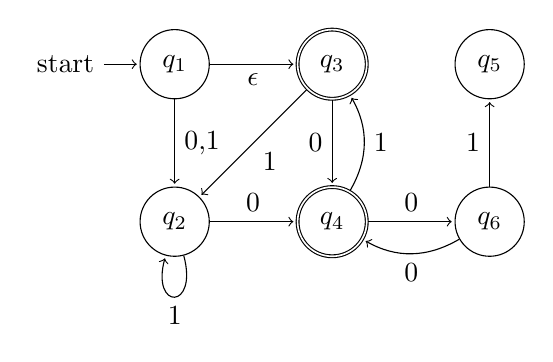
\begin{tikzpicture}[shorten >=1pt,node distance=2cm,on grid,auto]
   \node[state,initial] (q_1)   {$q_1$};
   \node[state] (q_2) [below=of q_1] {$q_2$};
   \node[state,accepting] (q_3) [right=of q_1] {$q_3$};
   \node[state,accepting](q_4) [right=of q_2] {$q_4$};
   \node[state] (q_5) [right=of q_3] {$q_5$};
   \node[state] (q_6) [right=of q_4] {$q_6$};
    \path[->]
    (q_1) edge  node {0,1} (q_2)
          edge  node [swap] {\(\epsilon\)} (q_3)
    (q_2) edge  node {0} (q_4)
          edge [loop below] node {1} ()
    (q_3) edge  node [swap] {0} (q_4)
          edge  node {1} (q_2)
    (q_4) edge  node {0} (q_6)
          edge  [swap, bend right] node {1} (q_3)
    (q_6) edge  [bend left] node {0} (q_4)
          edge  node {1} (q_5);
\end{tikzpicture}

\caption{A six--state NFA. \label{fig:N_6}}
\end{figure}

A \textbf{DFA} expression is of the form
\begin{snippet}
DFA[numStates, alphabet, transitionMatrix,
    acceptStates, initialState]
\end{snippet}
The number of states is a nonnegative integer; any DFA with zero states
accepts no words.
The alphabet is a sorted list of distinct strings, not containing
\codefont{""}.
A value of \codefont{\{\}}
means the DFA accepts either the empty language or \( \{ \epsilon \} \).
The transition matrix is a \codefont{numStates} by
\codefont{Length[alphabet]} matrix where entry \( i,j \) is the
state accessible from state \( i \) and letter \codefont{alphabet[[j]]}.
If the number of states is zero, then \codefont{transitionMatrix == \{\}}.
If the alphabet is empty, then \codefont{transitionMatrix ==
  \{\{\}, \{\}, ...\}}.
The accept states are a list of integers between \( 1 \) and the
number of states.
The initial state is an integer between \( 1 \) and the number of states, or
\codefont{Null} if \codefont{numStates ==  0}.

As an example, we can represent the DFA shown in Figure \ref{fig:D_5}
with the following expression.

\begin{snippet}
DFA[5, {"0", "1"}, {
    {2, 3},
    {2, 4},
    {4, 3},
    {5, 5},
    {5, 5}
}, {4}, 1]
\end{snippet}

A regular expression that is equivalent to the DFA in Figure \ref{fig:D_5} is
\[ (0(0)^*1|1(1)^*0). \]

\begin{figure}
\centering

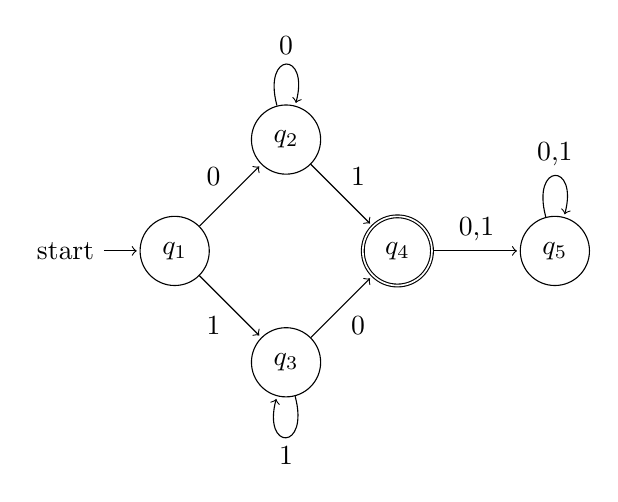
\begin{tikzpicture}[shorten >=1pt,node distance=2cm,on grid,auto]
   \node[state,initial] (q_1)   {$q_1$};
   \node[state] (q_2) [above right=of q_1] {$q_2$};
   \node[state] (q_3) [below right=of q_1] {$q_3$};
   \node[state,accepting](q_4) [below right=of q_2] {$q_4$};
   \node[state] (q_5) [right=of q_4] {$q_5$};
    \path[->]
    (q_1) edge  node {0} (q_2)
          edge  node [swap] {1} (q_3)
    (q_2) edge  node  {1} (q_4)
          edge [loop above] node {0} ()
    (q_3) edge  node [swap] {0} (q_4)
          edge [loop below] node {1} ()
    (q_4) edge  node {0,1} (q_5)
    (q_5) edge [loop above] node {0,1} ();
\end{tikzpicture}

\caption{A five--state DFA. \label{fig:D_5}}
\end{figure}

In Genfunlib, a \textbf{regular expression} is represented by an expression
with head \codefont{Regex}, and an argument built up from nonempty strings,
\codefont{EmptyWord},
\codefont{RegexStar}, \codefont{RegexConcat}, and \codefont{RegexOr}.
The expression \codefont{Regex[Null]} matches no words (the empty language).

As an example, the regular expression \( (a|bb)^*bbb \) is represented as

\begin{snippet}
Regex[RegexConcat[RegexStar[RegexOr["a", RegexConcat["b", "b"]]],
    "b", "b", "b"]]
\end{snippet}

Applying Mathematica's \codefont{TreeForm} command to this expression produces
Figure \ref{fig:regextree}.

\begin{figure}
  \centerline{\includegraphics[width=300px]{regextree}}
\caption{The parse tree of \( (a|bb)^*bbb \). \label{fig:regextree}}
\end{figure}

\textbf{Right regular grammars} are represented in Genfunlib by expressions
with head
\codefont{RRGrammar}, and one argument which is a list of rules in the form
\codefont{sym -> RHS} or \codefont{sym[n] -> RHS}, where
\codefont{sym} is a symbol,
\codefont{n} is an integer, and
\codefont{RHS} is either
\begin{itemize}
    \item \codefont{EmptyWord},
    \item a string,
    \item an expression on the left hand side of another rule,
    \item \codefont{RRGrammarConcat[str, sym]} (where \codefont{str} is a
      string),
    \item \codefont{RRGrammarConcat[str, sym[n]]}, or
    \item \codefont{RRGrammarOr[args]}, where \codefont{args} is a sequence
      of any of the things in this list.
\end{itemize}
      Strings cannot be empty.
    An empty list corresponds to the empty language.

For example, let \( G \) be the right regular grammar such that
\(N = \{ S, A \} \), \( \Sigma = \{a, b, c\} \), and the production rules \(P\)
are
\begin{align*}
  S &\rightarrow aS\\
  S &\rightarrow bA\\
  A &\rightarrow \epsilon\\
  A &\rightarrow cA.
\end{align*}

It can be seen that \( G \) is equivalent to the regular expression
\( a^*bc^*. \)
In Genfunlib, \( G \) becomes
\begin{snippet}
RRGrammar[{
    s -> RRGrammarConcat["a", s],
    s -> RRGrammarConcat["b", a],
    a -> EmptyWord,
    a -> RRGrammarConcat["c", a]
}]
\end{snippet}

A \textbf{directed graph with labeled vertices} is represented by an
expression of the form
\codefont{Digraph[graph, startVertices, endVertices, eAccepted]}.
The graph is a directed Mathematica \codefont{Graph}, whose vertices are
all labeled with nonempty strings.
The starting vertices are a list of vertices of the graph; if this list is
empty, the language associated with the graph contains no words except
possibly \( \epsilon \).
The ending vertices are a list of vertices of the graph; if this list is
empty, the language associated with the graph contains no words except
possibly \( \epsilon \).
Finally, \codefont{eAccepted} is \codefont{True} if \( \epsilon \) is accepted
and \codefont{False} otherwise.\\

Any of the five RLRs can be converted to any other using the commands
\codefont{ToNFA}, \codefont{ToDFA}, \codefont{ToRegex}, \codefont{ToRRGrammar},
and \codefont{ToDigraph}.

\begin{snippet}
In[34]:= ?ToDFA
ToDFA[NFA[...]] is a DFA defined from a NFA.
ToDFA[Regex[...]] is a DFA defined from a symbolic regular
    expression.
ToDFA[RRGrammar[...]] is a DFA defined from a right
    regular grammar.
ToDFA[Digraph[...]] is a DFA defined from a digraph
    with labeled vertices.

In[35]:= ToDFA[Regex[RegexOr["a", RegexStar["b"]]]]

Out[35]= DFA[4, {"a", "b"}, {{2, 3}, {4, 4}, {4, 3}, {4, 4}}, {1, 2,
    3}, 1]
\end{snippet}

The algorithms for performing these conversions come from the textbook of
Sipser \cite{sipser} with two exceptions.
First, given an NFA \( M \) with state set \( Q, \) the standard algorithm for
obtaining a DFA that is equivalent to \( M \) involves computing the powerset
\( 2^Q \), which is used as the state set for the DFA.
In some cases, there is no DFA equivalent to \( M \) with a state set with
fewer elements than \( 2^Q \) \cite{shallit2009second}.
However, the algorithm used in Genfunlib produces an automaton with many fewer
states, when this is possible.
The first step is to remove states from the NFA that are inaccessible from
the start state or from every accepting state.
Each state removed halves the maximum size of the resulting DFA.
Next, when computing the set of states for the DFA, Genfunlib only includes
those sets in \( 2^Q \) that are accessible from the initial state by performing
an incremental search starting at the initial state.
Finally, the DFA is minimized using Hopcroft's algorithm \cite{sipser}.
Experimental tests showed a huge speed increase when using these steps to
avoid creating a DFA with \( 2^{|Q|} \) states.
In testing, Genfunlib found the minimal DFA of an NFA with \( 379 \) states
in under half an hour on a computer with an AMD Phenom II X4 995 CPU and \( 8 \)
gigabytes of RAM.
However, the resulting DFA had only \( 8 \) states, so in terms of the length
of the output, Genfunlib's performance still has room for improvement.
The dk.brics.automaton Java package \cite{brics} uses a similar determinization
algorithm, but the performance of that library is much higher than that of
Genfunlib, presumably because Java is a lower--level language than Mathematica.

The other somewhat unusual conversion algorithm used in Genfunlib is the one
that maps labeled digraphs to automata and vice versa, since the digraph RLR is
not included in textbooks on automata theory.
Because in Genfunlib's digraphs, vertices are labeled, and in the graphs
derived from automata, edges are labeled, something like the line digraph
construction can be used.
The \emph{line digraph} of a digraph \( G \) has one vertex for each edge
of \( G \), and has an edge between two of its vertices if and only if the
corresponding edges in \( G \) form a length--two directed path in \( G \).
``Graphs'' derived from automata are actually hypergraphs, but the line digraph
definition can be adapted to this case.
When Genfunlib converts something to a DFA, the output is a minimal DFA, but
when converting to labeled digraphs or NFAs, the output may not be minimal.
Minimizing NFAs is a PSPACE-complete problem \cite{pspace}.

As an illustration, the DFA in Figure \ref{fig:labeledDFA} has each of its
``edges'' shown with an integer label, in brackets.
Genfunlib converts this DFA to the digraph shown in Figure
\ref{fig:linedigraph}.
The vertices of this digraph are shown with extra labels in brackets indicating
the edge in the original DFA to which they correspond.

\begin{figure}
\centering

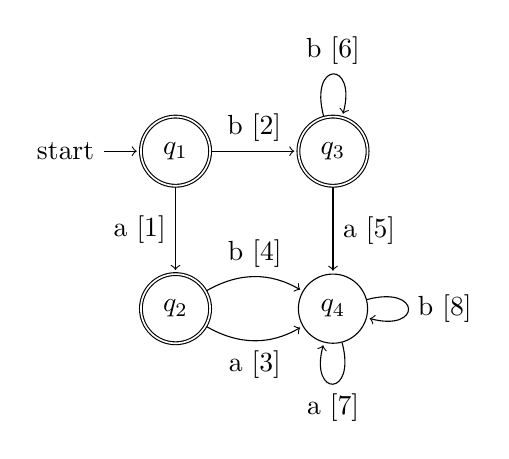
\begin{tikzpicture}[shorten >=1pt,node distance=2cm,on grid,auto]
   \node[state,initial,accepting] (q_1)   {$q_1$};
   \node[state,accepting] (q_2) [below=of q_1] {$q_2$};
   \node[state,accepting] (q_3) [right=of q_1] {$q_3$};
   \node[state] (q_4) [below=of q_3] {$q_4$};
    \path[->]
    (q_1) edge  node [swap] {a [1]} (q_2)
          edge  node {b [2]} (q_3)
    (q_2) edge  [bend right] node [swap] {a [3]} (q_4)
          edge  [bend left] node {b [4]} (q_4)
    (q_3) edge  node {a [5]} (q_4)
          edge [loop above] node {b [6]} ()
    (q_4) edge [loop below] node {a [7]} ()
          edge [loop right] node {b [8]} ();
\end{tikzpicture}

\caption{A DFA with eight transitions. \label{fig:labeledDFA}}
\end{figure}

\begin{figure}
\centering

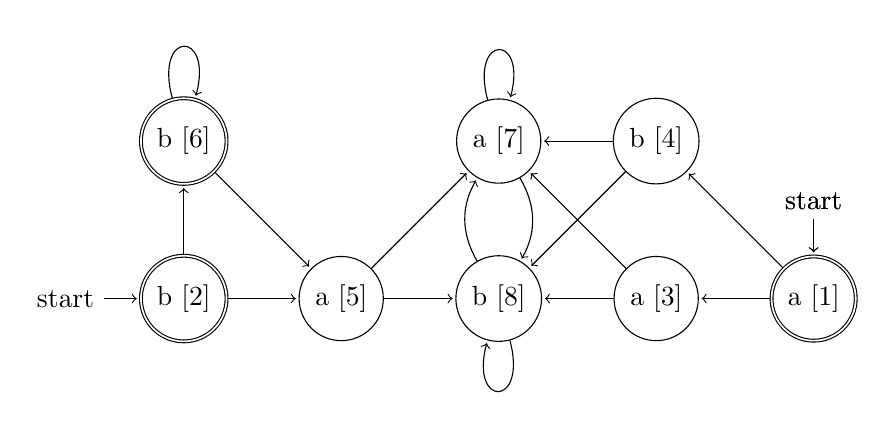
\begin{tikzpicture}[shorten >=1pt,node distance=2cm,on grid,auto]
  \node[state,initial,accepting] (q_2)  {b [2]};
  \node[state,accepting] (q_6) [above=of q_2] {b [6]};
  \node[state] (q_5) [right=of q_2] {a [5]};
  \node[state] (q_8) [right=of q_5] {b [8]};
  \node[state] (q_7) [above=of q_8] {a [7]};
  \node[state] (q_3) [right=of q_8] {a [3]};
  \node[state] (q_4) [right=of q_7] {b [4]};
  \node[state,initial,initial above,accepting] (q_1) [right=of q_3]  {a [1]};
    \path[->]
    (q_1) edge  node [swap] {} (q_3)
          edge  node {} (q_4)
    (q_2) edge  node [swap] {} (q_6)
          edge  node {} (q_5)
    (q_3) edge  node {} (q_7)
          edge  node {} (q_8)
    (q_4) edge  node {} (q_7)
          edge  node {} (q_8)
    (q_5) edge  node {} (q_7)
          edge  node {} (q_8)
    (q_6) edge  [loop above] node {} ()
          edge  node {} (q_5)
    (q_7) edge  [bend left] node {} (q_8)
          edge  [loop above] node {} ()
    (q_8) edge  [bend left] node {} (q_7)
          edge  [loop below] node {} ();
\end{tikzpicture}

\caption{The digraph constructed from the DFA in Figure \ref{fig:labeledDFA}.
Vertices are labeled by the transition they correspond to in the DFA.
\label{fig:linedigraph}}
\end{figure}

In addition to conversions between the five RLRs, Genfunlib includes functions
for converting between Genfunlib regular expressions and Mathematica built--in
regular expressions, which have head \codefont{RegularExpression}.
To be converted, the Mathematica regular expressions must have a restricted
syntax: Only letter characters, parentheses, asterisks, and bars (|) are
allowed.

The following example converts the regular expression \( (c|a)^* \) from
Mathematica syntax to Genfunlib syntax and back, and demonstrates how
built--in Mathematica functions such as \codefont{StringMatchQ} can be used
with Mathematica regular expressions.
\begin{snippet}
In[36]:= ToRegex[RegularExpression["(c|a)*"]]

Out[36]= Regex[RegexStar[RegexOr["c", "a"]]]

In[37]:= ToRegularExpression[%]

Out[37]= RegularExpression["((c|a))*"]

In[38]:= StringMatchQ["accaccccaaa", %]

Out[38]= True
\end{snippet}
Since, in Genfunlib, letters are represented by strings which may be longer
than one character (and words are represented by lists of strings), some issues
may arise when converting to Mathematica
regular expressions.
In Genfunlib, \codefont{\{"a","aa"\}} and \codefont{\{"aa","a"\}} are different
words.
However, since in Mathematica represents letters as length--one strings and
represented words as strings,
\begin{snippet}
Regex[RegexOr[RegexConcat["a", "aa"], RegexConcat["aa", "a"]]]
\end{snippet}
gets converted to
\begin{snippet}
RegularExpression["(aaa|aaa)"]
\end{snippet}

Regular languages have a rich set of closure properties \cite{sipser}, which
Genfunlib implements in the form of six operations:
Kleene star (\codefont{RegStar}),
complement (\codefont{RegComplement}),
reverse (\codefont{RegReverse}),
union (\codefont{RegUnion}),
concatenation (\codefont{RegConcat}), and
intersection (\codefont{RegIntersection}).

The algorithms for performing these operations all come from Sipser's textbook
\cite{sipser}.
For each operation, Genfunlib implements such an algorithm that works for one
type of RLR.
Then the operation is implemented for all other RLR types by converting them to
the type for which an algorithm is implemented, running the algorithm, then
converting back again.
As an example, the concatenation operation is directly implemented only for
right regular grammars, but users can call \codefont{RegConcat} on two DFAs
because they will get automatically converted to and from grammars.

The unary operations \codefont{RegStar} and \codefont{RegReverse} simply
take one RLR as an argument.
The operation \codefont{RegComplement} takes one RLR \(r\) and an alphabet
\( \Sigma \) and returns an RLR \( r' \) of the same type as \( r \) such that
\(L(r') = \Sigma^* \setminus L(r) \), where \( L(r) \) is the language of
\( r .\)
\begin{snippet}
In[39]:= ?RegComplement
RegComplement[NFA[...], {"str1", "str2",...}] performs the
    complement operation on an NFA with respect to a given
    alphabet.
RegComplement[DFA[...], {"str1", "str2",...}] performs the
    complement operation on a DFA with respect to a given
    alphabet.
RegComplement[Regex[...], {"str1", "str2",...}] performs the
    complement operation on a symbolic regular expression
    with respect to a given alphabet.
RegComplement[RRGrammar[...], {"str1", "str2",...}] performs the
    complement operation on a right regular grammar with respect
    to a given alphabet.
RegComplement[Digraph[...], {"str1", "str2",...}] performs the
    complement operation on a directed graph with respect to a
    given alphabet.

In[40]:= RegComplement[Regex[RegexStar["a"]], {"a", "b"}]

Out[40]= Regex[ RegexConcat[RegexStar["a"], "b",
    RegexStar[RegexOr["a", "b"]]]]
\end{snippet}
The binary operations \codefont{RegUnion}, \codefont{RegConcat}, and
\codefont{RegIntersection} take two RLRs of the same type.

Genfunlib overloads \codefont{GeneratingFunction} to take a regular expression
and a list of rules mapping letters to weights.
The regular expression is automatically disambiguated, and the letters are
replaced with their weights to obtain a rational power series.
Here we compute the generating function for the ambiguous regular expression
\( a|a|b|b^* \) that marks \( a \) with \( u \) and \(b \) with \( v \):

\begin{snippet}
In[41]:= GeneratingFunction[Regex[RegexOr["a","a","b",
    RegexStar["b"]]], {"a"->u,"b"->v}]
Out[41]= 1+u+v/(1-v)
\end{snippet}


\subsection{Symbolic method}
Genfunlib contains a basic implementation of the symbolic method.
An appropriate introduction to the symbolic method may be found in the author's
honours project \cite{honours} or Flajolet and Sedgewick's book \cite{flaj}.

Genfunlib allows combinatorial classes to be defined by specifications,
and can convert these specifications to corresponding systems of equations
in generating functions.

A specification is represented by an expression of the form
\begin{snippet}
Spec[{lhs1==rhs1,...},labeled?]
\end{snippet}
In the list of equations, the left hand sides are symbols representing classes,
and the right hand sides
are expressions built with combinatorial constructions, symbols
found in a left hand
side, restrictions (\codefont{Restricted[...]}),
and atomic and neutral classes.
The second argument is \codefont{True} if the classes are labeled, and
\codefont{False} if they are unlabeled.

Genfunlib supports multiple atomic classes, each of which is indexed by
a positive integer and is marked separately in generating functions.
They have the form \codefont{ZClass[1], ZClass[2],...}.
The neutral class is represented by the symbol \codefont{EClass}.

\begin{table}
  \centering
  \begin{tabular}{| l | l | l | l |}
    \hline
    \multicolumn{2}{|c|}{Labeled} & \multicolumn{2}{|c|}{Unlabeled} \\ \hline
    Sum            & \codefont{SMPlus} &   Sum & \codefont{SMPlus} \\ \hline
    Product       & \codefont{SMTimes} &  Product & \codefont{SMTimes} \\ \hline
    Sequence       & \codefont{SMSeq} &    Sequence & \codefont{SMSeq} \\ \hline
    Cycle           & \codefont{SMCyc} &    Cycle & \codefont{SMCyc} \\ \hline
    Set            & \codefont{SMSet} &    Powerset & \codefont{SMSet} \\ \hline
    Pointing & \codefont{SMPointing} & Multiset & \codefont{SMMultiset} \\\hline
    Substitution & \codefont{SMSub} & Pointing & \codefont{SMPointing} \\ \hline
    &  &    Substitution & \codefont{SMSub} \\ \hline
  \end{tabular}
  \caption{Admissible constructions supported by Genfunlib.}
  \label{tab:tabl}
\end{table}

The combinatorial constructions in Genfunlib are shown in Table \ref{tab:tabl},
along with their syntax.
Sum and product are commutative binary constructions;
sequence, cycle, set, multiset, and pointing are unary constructions.
Substitution is a binary construction, but it is not commutative.
The expression \codefont{SMSub[A,B]} corresponds to \( \mathcal{A}(\mathcal{B})
\), if \( \mathcal{A} \) is represented by the symbol \codefont{A} and
\( \mathcal{B} \) is represented by the symbol \codefont{B}.

The set, multiset, sequence, and cycle constructions take an optional second
argument in the form \codefont{Cardinality->f}, where \codefont{f} is a
predicate on the integers which gives the allowed number of components.
For example,
\begin{snippet}
SMSeq[class, Cardinality->(#<=k&)]
\end{snippet}
represents the class of finite sequences of elements of \codefont{class} with
at most \codefont{k} terms.
It is fine to use a symbol like \codefont{k} rather than an integer.

The other kind of restriction that can be done is with the
\codefont{Restricted} symbol.
The expression \codefont{Restricted[class,f]}, where \codefont{f} is a predicate
on the integers, represents the class of objects from \codefont{class}
with sizes that \codefont{f} maps to \codefont{True}.
For example,
\begin{snippet}
Restricted[SMSeq[SMTimes[ZClass[1],ZClass[2]]], #>2&]
\end{snippet}
represents the class containing all the objects in
\( \textsc{Seq}(\mathcal{Z}_1\times\mathcal{Z}_2) \) except the singleton
sequence.

\begin{mathematica}
  Predicates on the integers must return unevaluated when given symbolic input.
  The predicate \codefont{Mod[\#, 2]\&} satisfies this requirement, while
  \codefont{PrimeQ[\#]\&} does not.
\end{mathematica}

The command for passing from a combinatorial specification to a system
of generating function equations is \codefont{ToGFEqns}.
It takes two arguments, the first is a \codefont{Spec} expression and the second
is a symbol to be used as the indeterminate.
If the symbol \codefont{x} is supplied, \codefont{ZClass[1]} is marked with
\codefont{x[1]}, \codefont{ZClass[2]} is marked with \codefont{x[2]}, and so
on.
In the output, the generating function of a class is written as the symbol
for the class, with arguments.

\begin{snippet}
In[42]:= ?ToGFEqns
ToGFEqns[spec, indeterminate] gives the system of power series
equations corresponding to spec, using the given indeterminate.

In[43]:= ToGFEqns[
    Spec[{c == SMTimes[ZClass[1], SMSeq[ZClass[1]]]}, True], z]

Out[43]= {c[z[1]] == z[1]/(1 - z[1])}
\end{snippet}

The code that performs the translation to generating functions uses pattern
matching and replacement rules.
The following example snippet is a simplified segment of Genfunlib's code that
takes a specification called \codefont{spec} and replaces, e.g.\
\codefont{ZClass[2]} and \codefont{ZClass[3]} with \codefont{z[2]} and
\codefont{z[3]}, and replaces \codefont{EClass} with \codefont{1}.

\begin{snippet}
Replace[spec,
    {
        ZClass[n_] :> z[n],
        EClass :> 1,
    },
    {1, Infinity}, Heads -> True
];
\end{snippet}


Genfunlib includes one more command related to the symbolic method:
\codefont{ToGenfunlibSpec}.
This command takes two arguments.
The first is a string containing the Maple code for a Combstruct grammar in
the format used on the Encyclopedia of Combinatorial Structures (ECS)
website at
\begin{snippet}
http://algo.inria.fr/ecs/
\end{snippet}
The second argument is a Boolean value indicating whether the classes are
labeled.
The output is a \codefont{Spec} expression representing the same specification
as the Combstruct grammar.
Since Genfunlib and Combstruct specifications are similar in structure, the
conversion is not complex and mostly consists of term--for--term translation.
Class symbols are converted from upper case to lower case (and reduplicated)
to conform to Mathematica conventions.

As an example, we can take entry \#9 from the ECS: words on the alphabet
\(\{a,b\}\) with at most one consecutive \(b\)-letters.
The ECS gives the following unlabeled Combstruct specification:

\begin{snippet}
{S = Prod(X,Sequence(Prod(a,X))), X = Sequence(b,card <= 1),
    a = Atom, b = Atom }
\end{snippet}

In Genfunlib, the class \codefont{S} becomes \codefont{ss}.

\begin{snippet}
In[44]:= ?ToGenfunlibSpec
ToGenfunlibSpec[mapleString, labeled] converts from Combstruct to
    Genfunlib combinatorial specification syntax.

In[45]:= ToGenfunlibSpec["{S = Prod(X,Sequence(Prod(a,X))), X =
    Sequence(b,card <= 1), a = Atom, b = Atom }", False]

Out[45]= Spec[{ss == SMTimes[xx, SMSeq[SMTimes[a, xx]]],
    xx == SMSeq[b, Cardinality -> (#1 <= 1 &)], a == ZClass[1],
    b == ZClass[1]}, False]
\end{snippet}

We can convert to generating functions using indeterminate \codefont{z}
and solve for \codefont{ss[z[1]]}.

\begin{snippet}
In[46]:= ToGFEqns[%, z]

Out[46]= {ss[z[1]] == xx[z[1]]/(1 - a[z[1]] xx[z[1]]),
    xx[z[1]] == 1 + b[z[1]], a[z[1]] == z[1], b[z[1]] == z[1]}

In[47]:= Solve[Eliminate[%, {a[z[1]], b[z[1]], xx[z[1]]}],
    ss[z[1]]]

Out[47]= {{ss[z[1]] -> (-1 - z[1])/(-1 + z[1] + z[1]^2)}}
\end{snippet}

There is room for expansion of Genfunlib's symbolic method capabilities.
Symbolic method specifications are useful because tractable operations can
be performed on them.
This is of note since in general, combinatorial objects are too complex
for such simple notation.
Assuming the user is able to provide a combinatorial specification, one
valuable question may be whether the specification is well--formed.
The class \( \mathcal{I} \) defined by \( \mathcal{I} = \textsc{Seq}(
\mathcal{E}) \) has an infinite set of objects of size \( 0 \), so the
specification should be edited before anything is done with it.
Work on checking specifications for well--definedness has been published
by Salvy and coauthors \cite{auto,newsalvy}.
Genfunlib does not implement these complete validity checks on specifications;
however, errors are likely to be found at a later state when working with
power series.
For example,
\( \mathcal{I} = \textsc{Seq}( \mathcal{E}) \)
would generate a division by \( 0 \) error.

Lastly, there exists a notation system and framework for combinatorial objects
similar to symbolic combinatorics called species \cite{honours}.
Currently, Genfunlib provides support for the symbolic method only, although
the possibility of implementing species instead and including a converter
for specifications from the symbolic method to species was considered.
It does appear as though a natural mapping exists between the sequence,
set, and cycle constructions on the one hand, and the species of linear orders,
sets, and cyclic permutations on the other.
However, problems arise eventually.
Whereas the pointing construction in the symbolic method corresponds,
in unlabeled structures, to the power series operator \(xD\), for a species
\( F \) the type generating series \( \widetilde{F^\circ}(x) \) cannot be
expressed in terms of \( \widetilde{F}(x) \), but is given by
\[ \widetilde{F^\circ}(x) = x \left( \frac{\partial}{\partial x_1} Z_F \right)
  (x, x^2, x^3, \dots).
\]
Thus, in species, the pointing operation cannot correspond to any admissible
construction in the symbolic method.
This kind of subtle difference also exists between the substitution
``construction'' in the symbolic method and ``operation'' in species.
Salvy et al.\ discuss perhaps less serious issues with converting the
unlabeled multiset construction to the language of species \cite{newsalvy}.

\subsection{Asymptotics} \label{sub:asympt}

Flajolet et al.\ \cite{auto} define the class \( \mathcal{E} \) of
\emph{elementary functions} as the set of functions containing the
monomials \(1\) and \( z, \) and closed under the operations
of \( \{+,\times,Q,L,E \}, \) where
\[ Q(f)=\frac{1}{1-f}, \ \ L(f)=\log\frac{1}{1-f}, \ \ E(f)=\exp(f). \]
They proceed to give algorithms that can be used to automatically extract
Maclaurin coefficient asymptotics for functions in a subset of
\( \mathcal{E}.  \)
Before going further here, we note that at this point some confusion can appear
related to the terminology and notation used.
First, even though when talking about asymptotics we need to think of
generating functions as complex functions, for the purpose of computer
algebra we really still compute with power series.
That is, ``\( \exp(z) \)'' cannot, strictly speaking, be called a function.
Also, we actually want to talk about \emph{expressions}
built with the operations \( +, \times, Q, L, E, \) etc.\ --- we are talking
about syntax, not semantics.
Deciding whether a given expression semantically belongs in \( \mathcal{E} \)
is in general impossible, and not our main goal.

The class \( \mathcal{E} \) is subdivided into three disjoint sets
\[ \mathcal{E} = \mathcal{E}_{\text{AL}} \hspace{3pt} \dot{\cup} \hspace{3pt}
    \mathcal{E}_{\text{entire}} \hspace{3pt} \dot{\cup} \hspace{3pt}
    \mathcal{E}_{\text{other}}, \]
where \( \mathcal{E}_{\text{entire}} \) is the set of functions in
\( \mathcal{E} \) that are entire, and \( \mathcal{E}_{\text{AL}} \) is the
functions with \emph{algebraic--logarithmic} growth, meaning that \( f \in
\mathcal{E}_{\text{AL}} \) if and only if \( f \) has radius of convergence \(
0 < r < \infty \) then there exist
\( \alpha \in \mathbb{R}, k \in \mathbb{Z}_{\geq 0} \)
such that
\[ f(z) \sim \frac{1}{(1-z/r)^\alpha} \log^k \frac{1}{1-z/r}, \qquad \text{as }
z \rightarrow r^{-}. \]
The algorithm for computing asymptotic expansions of the Maclaurin coefficients
of functions in \( \mathcal{E}_{\text{AL}} \) described by Flajolet et al.\
\cite{auto} was implemented in Combstruct for Maple and is now partly
implemented in Genfunlib for Mathematica as the \codefont{CoefLimit} command.
This command takes an aperiodic function \( f \in \mathcal{E}_{\text{AL}} \) and
returns something asymptotically equivalent to the general term of the
Maclaurin coefficient sequence of \( f. \)
By saying that \( f \) is aperiodic, we mean that \( f(z) \) cannot be expressed
as \( z^a g(z^b) \) where \(b>1 \) and \( a \) are integers, and \( g \in
\mathcal{E}_{\text{AL}}.\)

\begin{snippet}
In[48]:= ?CoefLimit
CoefLimit[f,z,n] gives an expression that is asymptotically
    equivalent to SeriesCoefficient[f, {z,0,n}] as n goes to
    infinity.

In[49]:= CoefLimit[1/(1 - z*Exp[z]), z, n]

Out[49]= ProductLog[1]^(-1 - n)/(1 + E^ProductLog[1])

In[50]:= CoefLimit[1/(1 - Log[1/(1 - z*Exp[z])]), z, n]

Out[50]= -(((1 - (-1 + E)/E) ProductLog[(-1 + E)/E]^(-1 -
   n))/(-((-1 + E)/E) - E^ProductLog[(-1 + E)/E]))
\end{snippet}

In the case where \( f \in \mathcal{E}_{\text{AL}} \) has positive radius of
convergence \( r \) and
\[ f(z) \sim \frac{1}{(1-z/r)^\alpha} \log^k \frac{1}{1-z/r} \qquad \text{as }
z \rightarrow r^{-}, \]
where \( \alpha \leq 0, \) \codefont{CoefLimit} merely returns the exact
expression for the coefficients, using Mathematica's
\codefont{SeriesCoefficient}.

\begin{snippet}
In[51]:= CoefLimit[Log[1/(1 - z*Exp[z])], z, n]

Out[51]= SeriesCoefficient[Log[1/(1 - E^z z)], {z, 0, n}]

In[52]:= $Assumptions = n > 1;

In[53]:= CoefLimit[1/(1 - z) Log[1/(1 - 2 z)], z, n]

Out[53]= -I*Pi - 2^(1 + n) LerchPhi[2, 1, 1 + n]
\end{snippet}
Here \codefont{LerchPhi[2, 1, 1 + n]} represents \( \sum_{k \geq 0}
2^k/(k+n+1). \)


\begin{mathematica}
  The original algorithm \cite{auto} works for periodic generating functions
  and can obtain an asymptotic expansions of the form
  \[ C \rho^{-n} n^s \log^k n \left(1 + O\left(\frac{1}{\log n} \right) \right).
  \]
  However, in Mathematica asymptotic series are represented with
  \codefont{SeriesData} objects, and these only support big--Oh terms of the
  form \( O(n^k). \)
  Thus, \codefont{CoefLimit} does not give big--Oh terms, merely the
  dominant term.
  Since periodic generating functions have zeroes in their coefficients,
  the coefficients are not asymptotically equivalent to anything, so Genfunlib
  cannot give an asymptotic expression in this case.
\end{mathematica}

A general way to specify a generating function is to define it implicitly
by a power series equation.
Genfunlib provides the \codefont{TreeAsymptot} command for computing the
coefficient asymptotics of generating functions \( f(z) \) satisfying equations
of the form
\[ f(z) = z \phi(f(z)), \]
where \( \phi \in \mathcal{E}_{\text{AL}} \) satisfies
\( \phi(z) \neq c_0 + c_1 z \) and
\( \phi(0) \neq 0.\)
In this case, we can apply Theorem VI.6 \cite{flaj} to derive the asymptotics
of \( [z^n]f(z) \) provided we can compute
the minimum solution \( \tau \) to the characteristic equation
\[ \phi(\tau) - \tau \phi'(\tau) = 0, \qquad \tau > 0, \]
and the periodicity of \( \phi \).
The value of \( \tau \) can be computed by Mathematica's built--in equation
solver, and we can obtain the necessary information about the period of \( \phi
\) via the ``Reduction'' algorithm from Flajolet et.\ al \cite{auto}.

The \codefont{TreeAsymptot} command uses this method to give an asymptotic
expression consisting of a main estimate and a big O term.

\begin{snippet}
In[54]:= ?TreeAsymptot
TreeAsymptot[y[z]==z*phi,n] gives an asymptotic series for
    SeriesCoefficient[y[z], {z,0,n}] as n goes to infinity,
    where y[z] is the solution to y[z]==z*phi that is
    analytic at 0.

In[55]:= TreeAsymptot[f[z] == z*Exp[f[z]], n]

Out[55]= E^n ( (n^(-1))^(3/2)/Sqrt[2*Pi] + O[1/n]^(5/2))
\end{snippet}

The case where \( \phi(z) \) is periodic is allowed.

\begin{snippet}
In[56]:= TreeAsymptot[f[z] == z*Exp[f[z]^2], n]

Out[56]= (2 E)^(n/2) Boole[Mod[n, 2] == 1] ((n^(-1))^(3/2)/
    Sqrt[2*Pi] + O[1/n]^(5/2))
\end{snippet}

Flajolet and Sedgewick \cite{flaj} give an algorithm for obtaining coefficient
asymptotics of generating functions defined by algebraic equations.
This surely useful algorithm has so far not been implemented in any computer
algebra system.

\section{Genfunlib in action} \label{sec:action}

\subsection{Mathematics contest problems} \label{sec:contest}

Elementary problems from combinatorics are often chosen for high school math
contests.
This subsection contains a selection of contest--style problems and shows how
Genfunlib can help to solve them;
more contest problems solved with the aid of a computer algebra system can be
found in an article by Dumas and Salvy \cite{putnam}.

\begin{prob}
  How many arrangements are there of the letters in the word MATHEMATICS?
  \cite{pretest}
\end{prob}

\begin{sol}
As Zeilberger says \cite{companion}, ``Enumerating specific finite sets is no
longer considered mathematics.
A genuine mathematical fact has to incorporate
infinitely many facts, and the generic enumeration problem is to enumerate not
just one set but all the sets in an infinite family.''
In particular, this problem can be solved easily ``by computer'' simply by
performing a brute--force enumeration (in a math contest, this method is too
slow).
However, Genfunlib could also be used.

  The word MATHEMATICS contains \( 11 \) letters.
  If we create sequences of \( 11 \) atoms \( \circled{1}, \) we can associate
  the label of the \( i \)th atom with the position of the \( i \)th letter
  of MATHEMATICS in an arrangement of the letters.
  For example,
  \[
    \left( \circled{8}, \circled{4}, \circled{5}, \circled{2}, \circled{7},
    \circled{1}, \circled{3}, \circled{10}, \circled{9}, \circled{11},
  \circled{6} \right) \]
  corresponds to the arrangement MHAATSEMITC.
  The problem is that not all letters in MATHEMATICS are distinct, so not every
  different labeled sequence corresponds to a different arrangement.
  We fix this by creating sequences of sets of atoms, where there is one set
  for each different letter in MATHEMATICS.
  This way, each set of positions of a letter is counted, not each sequence of
  positions.

  Our specification of the class \( \mathcal{M} \) of rearrangements of
  MATHEMATICS is
  \begin{align*}
    \mathcal{M} &= \textsc{Set}_2 \left(\circled{1} \right)^3 \times
    \textsc{Set}_1 \left( \circled{1} \right)^5 \\
        &= \textsc{Set}_2 \left(\circled{1} \right)^3 \times \circled{1}^5.
  \end{align*}
  With Genfunlib, we convert this to an exponential generating function
  \codefont{m[z]} where
  the coefficient of \( z^{11} \) multiplied by \( 11! \) is the solution to
  the problem.
  \begin{snippet}
In[57]:= ToGFEqns[Spec[{
    m == SMTimes[
    SMSet[ZClass[1], Cardinality -> (# == 2 &)],
    SMSet[ZClass[1], Cardinality -> (# == 2 &)],
    SMSet[ZClass[1], Cardinality -> (# == 2 &)],
    ZClass[1],
    ZClass[1],
    ZClass[1],
    ZClass[1],
    ZClass[1]
    ]}, True], z] /. z[1] -> z

Out[57]= {m[z] == z^11/8}
\end{snippet}
From here we observe that the solution is
\begin{snippet}
In[58]:= 11!/8

Out[58]= 4989600
\end{snippet}
\end{sol}


\begin{prob} \label{prob:coins}
  A fair coin is to be tossed ten times.
  Find the probability that heads never occur on three consecutive tosses.
  (This is a modified version of AIME 1990 \#9, a typical Fibonacci problem
  \cite{jam}.)
\end{prob}

\begin{sol}
  Say the coin is tossed \( n \) times.
  Then we can represent the sequence of tosses as an \(n\)--word over the
  alphabet \( \{ H, T \}. \)
  Let \( N \) be the NFA in Figure \ref{fig:Ncoins}.
Then the language accepted by \( N \) is the set of words representing coin
tosses in which heads never occur on three consecutive tosses.
Using Genfunlib, we can convert \( N \) to an equivalent regular expression.

\begin{figure}
\centering

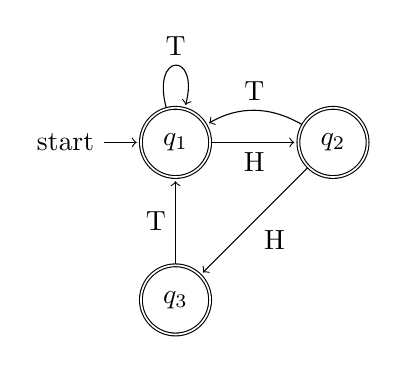
\begin{tikzpicture}[shorten >=1pt,node distance=2cm,on grid,auto]
   \node[state,initial,accepting] (q_1)   {$q_1$};
   \node[state,accepting] (q_2) [right=of q_1] {$q_2$};
   \node[state,accepting] (q_3) [below=of q_1] {$q_3$};
    \path[->]
    (q_1) edge  [loop above] node {T} ()
          edge  node [swap] {H} (q_2)
    (q_2) edge  [bend right, swap] node  {T} (q_1)
          edge  node {H} (q_3)
    (q_3) edge  node {T} (q_1);
\end{tikzpicture}

\caption{An NFA \( N \) for the allowed sequences of coin tosses in Problem
  \ref{prob:coins}. \label{fig:Ncoins}}
\end{figure}

\begin{snippet}
In[59]:= ToRegex[NFA[3,{"H","T"},{
    {{2},{1},{}},
    {{3},{1},{}},
    {{},{1},{}}
    },{1,2,3},1]]

Out[59]= Regex[RegexOr[RegexStar["T"],
    RegexConcat[RegexStar["T"], "H",
    RegexStar[RegexConcat["T", RegexStar["T"], "H"]],
    RegexOr[EmptyWord, RegexConcat["T", RegexStar["T"]]]],
    RegexConcat[RegexStar["T"], "H",
    RegexStar[RegexConcat["T", RegexStar["T"], "H"]], "H",
    RegexStar[
    RegexConcat["T", RegexStar["T"], "H",
    RegexStar[RegexConcat["T", RegexStar["T"], "H"]], "H"]],
    RegexOr[EmptyWord, RegexConcat["T", RegexStar["T"]],
    RegexConcat["T", RegexStar["T"], "H",
    RegexStar[RegexConcat["T", RegexStar["T"], "H"]],
    RegexOr[EmptyWord, RegexConcat["T", RegexStar["T"]]]]]]]]
\end{snippet}

Now, we obtain the generating function of this regular expression to find the
number of words of length \( 10. \)

\begin{snippet}
In[60]:= GeneratingFunction[%, {"H" -> z, "T" -> z}]

Out[60]= (1 + z (1 + z))/(1 - z - z (z + z^2))

In[61]:= SeriesCoefficient[%, {z, 0, 10}]

Out[61]= 504
\end{snippet}

Thus, the answer is \( 504/2^{10} = 63/128. \)
\end{sol}

\begin{prob}
  Find a recursion for the number of partitions of an \( n \)--set
  \cite{engel}.
\end{prob}

\begin{sol}
First we can note that the combinatorial class \( \mathcal{P} \) of set
partitions is defined
\[
  \mathcal{P} = \textsc{SMSet}\left(\textsc{SMSet}_{\geq 1}(\circled{1})
  \right).
\]
That is, a set partition is simply a set of nonempty sets.
With Genfunlib we can get the exponential generating function \( P(z) \) for
the class \( \mathcal{P}, \) represented by \codefont{p[z]}.

\begin{snippet}
In[62]:= ToGFEqns[
    Spec[{p == SMSet[SMSet[ZClass[1], Cardinality ->
    (# >= 1 &)]]}, True], z] /. z[1] -> z

Out[62]= {p[z] == E^(-1 + E^z)}
\end{snippet}
This is actually an explicit equation for the generating function
\codefont{p[z]}.
To arrive at a recurrence relation, we logarithmically differentiate both
sides and solve for \codefont{p[z]}.

\begin{snippet}
In[63]:= Solve[D[Log[p[z]], z] == D[Log[E^(-1 + E^z)], z], p[z]]

Out[63]= {{p[z] -> E^-z p'[z]}}
\end{snippet}

Using Genfunlib's enhancement to \codefont{SeriesCoefficient}, we extract
coefficients of the right hand side.

\begin{snippet}
In[64]:= SeriesCoefficient[E^-z p'[z], {z, 0, n}]

Out[64]= Sum[((-1)^$6*(1 + n - $6)*SeriesCoefficient[p[z],
    {z, 0, 1 + n - $6}, Assumptions -> Element[$6, Integers] &&
    $6 >= 0])/$6!, {$6, 0, n}]
\end{snippet}

If we let \( p_n = n! [z^n] P(z), \) we can use the above result to arrive at
the relation
\[
  p_0=1, \qquad p_n = p_{n-1} - \sum_{j=1}^{n-1} \binom{n-1}{j} (-1)^j p_{n-j}.
\]
\end{sol}

\begin{prob}
  Prove that the number of binary \(n\)--words with exactly \( m \) \(01\)--
  blocks is \( \binom{n+1}{2m+1} \) \cite{engel}.
\end{prob}

\begin{sol}
  The way we attack this problem is defining the NFA \( N_b \) in Figure
  \ref{fig:b}.
  The language that \( N_b \) accepts is all words over the alphabet
  \( \{ 0, 1, b \} \) where the letter \( b \) only appears as part of the
  subword \( 0b1, \) and the subword \( 01 \) never appears.
  Counting the number of words with \(n \) letters \(0\) and \(1\) and
  \(m \) occurrences of \( b \) will solve the problem.

\begin{figure}
\centering

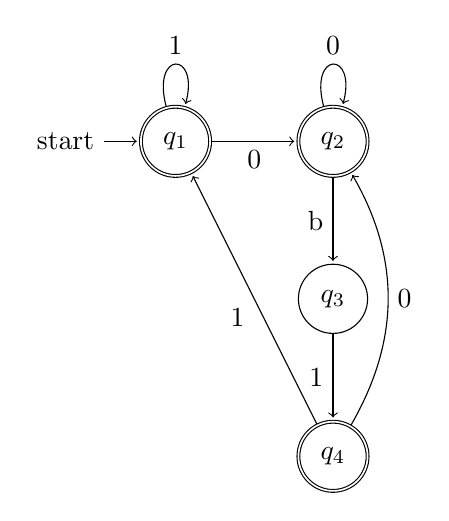
\begin{tikzpicture}[shorten >=1pt,node distance=2cm,on grid,auto]
   \node[state,initial,accepting] (q_1)   {$q_1$};
   \node[state,accepting] (q_2) [right=of q_1] {$q_2$};
   \node[state] (q_3) [below=of q_2] {$q_3$};
   \node[state,accepting] (q_4) [below=of q_3] {$q_4$};
    \path[->]
    (q_1) edge  [loop above] node {1} ()
          edge  node [swap] {0} (q_2)
    (q_2) edge  [swap] node {b} (q_3)
          edge  [loop above] node {0} ()
    (q_3) edge  [swap]node {1} (q_4)
    (q_4) edge  [bend right, swap] node {0} (q_2)
          edge  node {1} (q_1);
\end{tikzpicture}

\caption{An NFA \( N_b \) that marks \(01\) blocks with \(b\). \label{fig:b}}
\end{figure}

  We define \codefont{nfab} to be \( N_b \) from Figure \ref{fig:b} with
  Genfunlib.

  \begin{snippet}
In[65]:= nfab = NFA[4, {"0", "1", "b"}, {
    {{2}, {1}, {}, {}},
    {{2}, {}, {3}, {}},
    {{}, {4}, {}, {}},
    {{2}, {1}, {}, {}}
    }, {1, 2, 4}, 1];
  \end{snippet}

  We obtain a generating function from \codefont{nfab}, with \( u \)
  marking \( 0 \) and \( 1 \), and \( v \) marking \( b. \)

  \begin{snippet}
In[66]:= GeneratingFunction[ToRegex[nfab],
    {"0" -> u, "1" -> u, "b" -> v}]

Out[66]= (1 + u/(1 - u))/(1 - u - (u^2 v)/(1 - u))
\end{snippet}

  Now, we extract the coefficient of \( v^m. \)

  \begin{snippet}
In[67]:= $Assumptions = m >= 0;

In[68]:= SeriesCoefficient[1/(1 + u (-2 + u - u v)), {v, 0, m}]

Out[68]= (u^2/(-1 + u)^2)^(1 + m)/u^2
\end{snippet}

Lastly we compare this to \( \sum_{n \geq 2m} \binom{n+1}{2m+1} u^n. \)

\begin{snippet}
In[69]:= Out[68] == Sum[Binomial[n + 1, 2 m + 1] u^n,
    {n, 2 m, Infinity}] // FullSimplify

Out[69]= True
\end{snippet}

This may seem like an indirect route to the result.
The explanation is that, as long as we want to use Mathematica and Genfunlib
as much as possible, the most direct route sometimes does not work but
something more creative does.
\end{sol}

\begin{prob}
  How many \(n\)--words from the alphabet \( \{0,1,2 \} \) are such that the
  neighbors differ by at most \( 1 \)? \cite{engel}
\end{prob}

\begin{sol}
  One can see that this is a regular language accepted by the NFA \(N_d\) shown
  in Figure \ref{fig:d}.
We define \( N_d \) in Genfunlib as \codefont{nfadif}.

\begin{figure}
\centering

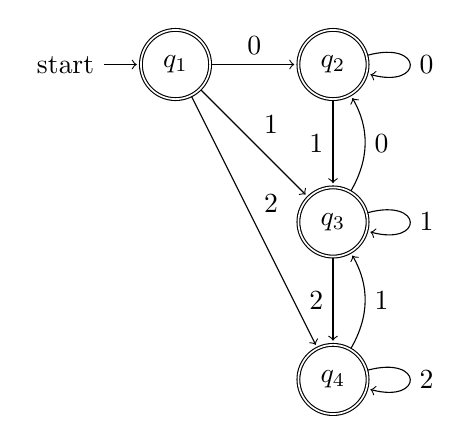
\begin{tikzpicture}[shorten >=1pt,node distance=2cm,on grid,auto]
   \node[state,initial,accepting] (q_1)   {$q_1$};
   \node[state,accepting] (q_2) [right=of q_1] {$q_2$};
   \node[state,accepting] (q_3) [below=of q_2] {$q_3$};
   \node[state,accepting] (q_4) [below=of q_3] {$q_4$};
    \path[->]
    (q_1) edge  node {0} (q_2)
          edge  node {1} (q_3)
          edge  node {2} (q_4)
    (q_2) edge  [swap] node {1} (q_3)
          edge  [loop right] node {0} ()
    (q_3) edge  [bend right,swap] node {0} (q_2)
          edge  [loop right] node {1} ()
          edge  [swap] node {2} (q_4)
    (q_4) edge  [loop right] node {2} ()
          edge  [bend right,swap] node {1} (q_3);
\end{tikzpicture}
\caption{The NFA \( N_d \) that accepts words from the alphabet \( \{0,1,2\} \)
such that neighboring letters differ by at most \( 1 \). \label{fig:d}}
\end{figure}

\begin{snippet}
nfadif = NFA[4, {"0", "1", "2"}, {
    {{2}, {3}, {4}, {}},
    {{2}, {3}, {}, {}},
    {{2}, {3}, {4}, {}},
    {{}, {3}, {4}, {}}
    }, {1, 2, 3, 4}, 1];
\end{snippet}

All that remains in order to count the \(n\)--words is to obtain the generating
function and extract coefficients.

\begin{snippet}
In[70]:= GeneratingFunction[
    ToRegex[nfadif], {"0" -> z, "1" -> z, "2" -> z}] //
    FullSimplify

Out[70]= -((1 + z)/(-1 + z (2 + z)))

In[71]:= $Assumptions = n >= 1;

In[72]:= SeriesCoefficient[-((1 + z)/(-1 + z (2 + z))), {z, 0, n}]

Out[72]= (-2 (1 - Sqrt[2])^n + Sqrt[2] (1 - Sqrt[2])^n +
    2 (1 + Sqrt[2])^n + Sqrt[2] (1 + Sqrt[2])^n)/(2 Sqrt[2])
\end{snippet}

Simplified and in standard mathematical notation, this says that there are
\[
\frac{1}{2} \left(\left(1-\sqrt{2}\right)^{n+1}+
    \left(1+\sqrt{2}\right)^{n+1}\right)
\]
\(n\)--words from the alphabet \( \{0,1,2\} \) such that neighboring letters
differ by at most \( 1. \)
\end{sol}

\begin{prob}
  If \( n \) people sit around a circular table, how many of the \( n! \)
  arrangements are distinct, i.e., do not have the same neighboring relations?
\end{prob}

\begin{sol}
  The first thing to note about this problem is that it appears to be
  ambiguous.
  Is the neighboring relation who is sitting next to whom, or who is sitting
  to the left of whom?
  Let us solve the problem for the latter case.
  It turns out that the final answers simply differ by a factor of \( 2. \)

  We represent the seating arrangements by the combinatorial class
  \( \mathcal{C} = \textsc{Cyc} \left(\circled{1} \right). \)
  That is, the objects in \( \mathcal{C} \) are labeled cycles.
  With Genfunlib, we can find \codefont{c[z]}, the generating function
  of \( \mathcal{C}, \) and extract coefficients.

  \begin{snippet}
In[73]:= ToGFEqns[Spec[{c == SMCyc[ZClass[1]]}, True], z]
    /. z[1] -> z

Out[73]= {c[z] == Log[1/(1 - z)]}

In[74]:= SeriesCoefficient[Log[1/(1 - z)], {z, 0, n}]

Out[74]= 1/n
\end{snippet}

Since \codefont{c[z]} is an exponential generating function, the number of
distinct arrangements is \( n! / n = (n-1)!. \)
\end{sol}

\begin{prob}
    A permutation \( p \) of the set \( \{1, \dots, n \} \) is called an
    \emph{involution} if \( p \circ p = \text{Id}. \)
    Find a recursion for the number \( t_n \) of involutions of
    \( \{1, \dots, n \}. \)
    Also find a closed formula in the form of a sum \cite{engel}.
\end{prob}

\begin{sol}
  The functional graph of an involution is a set of \(1\)-- and \(2\)--cycles.
  So we define the class \( \mathcal{G} \) by
  \[ \mathcal{G} = \textsc{Set} \left(\textsc{Cyc}_{\leq 2} \left( \circled{1}
    \right) \right). \]
  With Genfunlib, we find the generating function \codefont{g[z]} for
  \( \mathcal{G} \).

  \begin{snippet}
In[75]:= ToGFEqns[Spec[{g == SMSet[SMCyc[ZClass[1]],
    Cardinality -> (# <= 2 &)]}, True], z] /. z[1] -> z

Out[75]= {g[z] == 1 + Log[1/(1 - z)] + 1/2 Log[1/(1 - z)]^2}
\end{snippet}

From this expression for \codefont{g[z]}, Mathematica can produce a recurrence
relation for \(t_n\), which we call \codefont{tn}.
\begin{snippet}
In[76]:= tn = FullSimplify[ n! SeriesCoefficient[
    1 + Log[1/(1 - z)] + 1/2 Log[1/(1 - z)]^2, {z, 0, n}]];

In[77]:= DifferenceRootReduce[tn]

Out[77]= DifferenceRoot[
    Function[{y, n}, {n^2 y[n] + (-1 - 2 n) y[ 1 + n] +
    y[2 + n] == 0, y[1] == 1, y[2] == 2}]][n]
\end{snippet}
That is, \(t_1 = 1, t_2 = 2, \) and, for \( n \geq 3, \)
\[ n^2 t_n - (2n + 1)t_{n+1} + t_{n+2} = 0. \]

Now, finding a sum for \( t_n \) should be easy since we have the
generating function \codefont{g[z]}.
There is a small problem, though, which is that Mathematica tries to
``simplify'' the sum into something else as soon as it is obtained.
To avoid this, we replace \( \log(1/(1-z)) \) in \codefont{g[z]} with the
placeholder \( f(z), \) then extract coefficients from \codefont{g[z]} in terms
of the coefficients of \( f(z), \) using Genfunlib's enhancements to
Mathematica's \codefont{SeriesCoefficient}.
Then we replace coefficients of \( f(z) \) with the coefficients of
\( \log(1/(1-z)), \) and we are done.

\begin{snippet}
In[78]:= $FullAnalytic = True;

In[79]:= n! SeriesCoefficient[
  1 + Log[1/(1 - z)] + 1/2 Log[1/(1 - z)]^2 /.
   Log[1/(1 - z)] -> f[z], {z, 0, n}]

Out[79]=  n!*(SeriesCoefficient[f[z], {z, 0, n}] +
    Sum[SeriesCoefficient[f[z], {z, 0, n - $14}, Assumptions ->
    n >= 1 && Element[n, Integers] && Element[$14, Integers] &&
    $14 >= 0]*SeriesCoefficient[f[z], {z, 0, $14},
    Assumptions -> n >= 1 && Element[n, Integers] &&
    Element[$14, Integers] && $14 >= 0], {$14, 0, n}]/2)

In[80]:= % /. SeriesCoefficient[f[z], {z, 0, j_}, ___] :>
    Boole[j > 0]/j

Out[80]= n!*(Boole[n > 0]/n + Sum[(Boole[n - $14 > 0]*
    Boole[$14 > 0])/ ((n - $14)*$14), {$14, 0, n}]/2)
  \end{snippet}

  The result is a bit cluttered, but after a little inspection, it says that,
  for \( n \geq 1, \)
  \[ t_n = n! \left( \frac{1}{n} + \frac{1}{2} \sum_{j=1}^{n-1} \frac{1}{j(n-j)}
    \right). \]
\end{sol}

\begin{prob} \label{prob:neigh}
  Let \(f(n) \) be the number of \(n\)--words without neighboring zeros from
  the alphabet \( \{0, 1, 2\}. \)
  Find a recursion and a formula for \( f(n). \)
\end{prob}
\begin{sol}
  To specify the language of interest, we define the grammar \( G \) with
  the following productions.

\begin{align*}
  A &\rightarrow 1 \cdot A \\
  A &\rightarrow 2 \cdot A \\
  A &\rightarrow 0 \cdot B \\
  B &\rightarrow 1 \cdot A \\
  B &\rightarrow 2 \cdot A \\
  A &\rightarrow \epsilon \\
  B &\rightarrow \epsilon
\end{align*}

In Genfunlib, we can define the corresponding grammar \codefont{oneZero} and
compute the generating function.

\begin{snippet}
In[81]:= oneZero = RRGrammar[{
    a -> RRGrammarConcat["1", a],
    a -> RRGrammarConcat["2", a],
    a -> RRGrammarConcat["0", b],
    b -> RRGrammarConcat["1", a],
    b -> RRGrammarConcat["2", a],
    a -> EmptyWord,
    b -> EmptyWord}];

In[82]:= GeneratingFunction[ ToRegex[oneZero],
    {"0" -> z, "1" -> z, "2" -> z}]

Out[82]= (1 + z)/(1 - 2 z - 2 z^2)
\end{snippet}

Figure \ref{fig:graph} shows a digraph with labeled vertices corresponding to
\codefont{oneZero}, which was created with Genfunlib's \codefont{ToDigraph}
command and edited slightly for clarity.

\begin{figure}
  \centerline{\includegraphics[width=350px]{graph2}}
  \caption{A digraph with labeled vertices that is equivalent to the grammar \(
    G \) from Problem \ref{prob:neigh},
    which accepts words in \( \{0,1,2\}^* \) that avoid the subword \( 00. \)
    This non--minimal digraph was generated with the \codefont{ToDigraph}
    command and plotted using Mathematica's built--in functionality.
    Green vertices are start vertices, and vertices with dotted borders are
    accepting vertices.
    \label{fig:graph}}
\end{figure}

Finding a formula for \( f(n) \) is now as simple as extracting coefficients
using Mathematica's \codefont{SeriesCoefficient} command.

\begin{snippet}
In[83]:= SeriesCoefficient[%, {z, 0, n}]

Out[83]= (-2 (1 - Sqrt[3])^n + Sqrt[3] (1 - Sqrt[3])^n +
    2 (1 + Sqrt[3])^n + Sqrt[3] (1 + Sqrt[3])^n)/(2 Sqrt[3])
  \end{snippet}
  After some simplification, we have that
  \[ f(n) = \frac{1}{6} \left(3+2 \sqrt{3}\right) \left(1+\sqrt{3}\right)^n-
  \frac{1}{6} \left(2 \sqrt{3}-3\right) \left(1-\sqrt{3}\right)^n. \]

  Obtaining a recurrence relation is as easy as calling a Mathematica
  command called \codefont{DifferenceRootReduce} .
  \begin{snippet}
In[84]:= DifferenceRootReduce[%, n] // FullSimplify

Out[84]= DifferenceRoot[ Function[{y, n}, {-2 y[n] -
    2 y[1 + n] + y[2 + n] == 0, y[0] == 1, y[1] == 3}]][n]
   \end{snippet}
That is, \( f(0) = 1, f(1) = 3, \) and, for \( n \geq 2, \)
\[  f(n+2) = 2f(n) + 2f(n+1).\]
\end{sol}

\begin{prob}
  How many binary trees with \(n\) labeled leaves are there? \cite{engel}
\end{prob}

\begin{sol}

We assume that ``binary trees'' are rooted plane trees such that every node has
either \( 0 \) or \( 2 \) children.
We assume that these leaf--labeled binary trees are binary trees whose leaves
are uniquely labeled.
The task is to count how many leaf--labeled binary trees there are with \(n\)
leaves.
Figure \ref{fig:leaves} shows all leaf--labeled binary trees with \( 3 \)
leaves.

\begin{figure}
  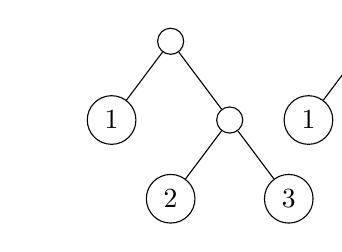
\begin{tikzpicture}[level distance=1cm]
    \node[circle,draw](z){}
    child{node[circle,draw]{1}}
    child{node[circle,draw]{}
      child{node[circle,draw] {2}} child{node[circle,draw] {3}} };

      \hspace{2.5cm}

    \node[circle,draw](z){}
    child{node[circle,draw]{1}}
    child{node[circle,draw]{}
      child{node[circle,draw] {3}} child{node[circle,draw] {2}} };

      \hspace{4cm}

    \node[circle,draw](z){}
    child{node[circle,draw]{}
      child{node[circle,draw] {1}} child{node[circle,draw] {2}} }
    child{node[circle,draw]{3}};

    \hspace{2.5cm}

    \node[circle,draw](z){}
    child{node[circle,draw]{}
      child{node[circle,draw] {1}} child{node[circle,draw] {3}} }
      child{node[circle,draw]{2}};
  \end{tikzpicture}\\

  \vspace{0.5cm}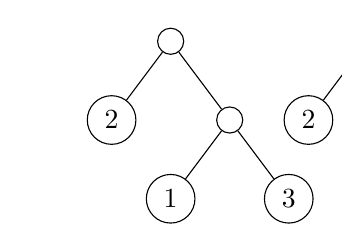
\begin{tikzpicture}[level distance=1cm]

    \node[circle,draw](z){}
    child{node[circle,draw]{2}}
    child{node[circle,draw]{}
      child{node[circle,draw] {1}} child{node[circle,draw] {3}} };

      \hspace{2.5cm}

    \node[circle,draw](z){}
    child{node[circle,draw]{2}}
    child{node[circle,draw]{}
      child{node[circle,draw] {3}} child{node[circle,draw] {1}} };

      \hspace{4cm}

    \node[circle,draw](z){}
    child{node[circle,draw]{}
      child{node[circle,draw] {2}} child{node[circle,draw] {1}} }
    child{node[circle,draw]{3}};

    \hspace{2.5cm}

    \node[circle,draw](z){}
    child{node[circle,draw]{}
      child{node[circle,draw] {2}} child{node[circle,draw] {3}} }
      child{node[circle,draw]{1}};
  \end{tikzpicture}\\

\vspace{0.5cm}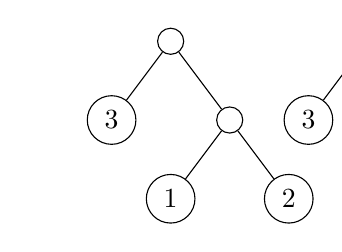
\begin{tikzpicture}[level distance=1cm]

    \node[circle,draw](z){}
    child{node[circle,draw]{3}}
    child{node[circle,draw]{}
      child{node[circle,draw] {1}} child{node[circle,draw] {2}} };

      \hspace{2.5cm}

    \node[circle,draw](z){}
    child{node[circle,draw]{3}}
    child{node[circle,draw]{}
      child{node[circle,draw] {2}} child{node[circle,draw] {1}} };

      \hspace{4cm}

    \node[circle,draw](z){}
    child{node[circle,draw]{}
      child{node[circle,draw] {3}} child{node[circle,draw] {1}} }
    child{node[circle,draw]{2}};

    \hspace{2.5cm}

    \node[circle,draw](z){}
    child{node[circle,draw]{}
      child{node[circle,draw] {3}} child{node[circle,draw] {2}} }
      child{node[circle,draw]{1}};
  \end{tikzpicture}

\caption{The \( 12\) binary trees with \(3\) labeled leaves. \label{fig:leaves}}
\end{figure}

First we define a combinatorial specification for the classes of leaves,
\( \mathcal{L}, \) inner nodes \( \mathcal{I}, \) and trees \( \mathcal{T}. \)
\begin{align*}
  \mathcal{L} &= \circled{1} \\
  \mathcal{I} &= \mathcal{E} \\
  \mathcal{T} &= \mathcal{L} + \mathcal{T} \times \mathcal{I} \times \mathcal{T}
\end{align*}

In Genfunlib, we can convert this specification to equations in the exponential
generating functions \codefont{l[z]} for \( \mathcal{L}, \) \codefont{i[z]}
for \( \mathcal{I}, \) and \codefont{t[z]} for \( \mathcal{T}. \)

\begin{snippet}
In[85]:= ToGFEqns[Spec[{
    l == ZClass[1],
    i == EClass,
    t == SMPlus[l, SMTimes[t, i, t]]
    }, True], z] /. z[1] -> z

Out[85]= {l[z] == z, i[z] == 1, t[z] == l[z] + i[z] t[z]^2}
\end{snippet}

We use Mathematica's \codefont{Eliminate} to provide us with an equation
in just our generating function of interest, \codefont{t[z]}.
\begin{snippet}
In[86]:= eqn = Eliminate[%, {l[z], i[z]}]

Out[86]= (1 - t[z]) t[z] == z
\end{snippet}

The power series equation \( (1-T(z))T(z) = z \) has two solutions in general,
but only one with nonnegative coefficients: \((1/2) \left(1-\sqrt{1-4 z}
\right). \)
Extracting coefficients with Mathematica's \codefont{SeriesCoefficient}
and multiplying by \( n! \) gives the final answer for the number of
leaf--labeled binary trees with \( n \) leaves.

\begin{snippet}
In[87]:= $Assumptions = n >= 1;

In[88]:= n! SeriesCoefficient[1/2 (1 - Sqrt[1 - 4 z]),
    {z, 0, n}]

Out[88]= -(-1)^n 2^(-1 + 2 n) Binomial[1/2, n] n!
\end{snippet}

Mathematica reports here that the formula is
\[ -(-1)^n 2^{2 n-1} n! \binom{\frac{1}{2}}{n}, \]
which is just a more cumbersome form of the expected result
\[\frac{(2 (n-1))!}{(n-1)!}. \]

We note that one way to come up with the specification in this solution is to
find the counting
sequence for leaf--labeled binary trees in the Encyclopedia of Combinatorial
Objects at \url{http://algo.inria.fr/ecs}.
It is entry number 51, ``Labelled Plane Binary Trees''.
The Encyclopedia shows the unlabeled Maple--syntax specification
\codefont{\{S = Union(Z,Prod(S,S))\}}, which we can use to get a specification
in Genfunlib via the \codefont{ToGenfunlibSpec} command.

\begin{snippet}
In[89]:= ToGenfunlibSpec["{S = Union(Z,Prod(S,S))}", False]

Out[89]= Spec[{ss == SMPlus[ZClass[1], SMTimes[ss, ss]]}, False]
\end{snippet}


\end{sol}

\begin{prob}
  Let \( k \) and \( n \) be integers such that \(1 \leq k \leq n. \)
  Consider all finite sequences of positive integers with sum \( n. \)
  Suppose that the term \( k \) occurs \(T(n,k)\) times in all these
  sequences.
  Find \( T(n,k). \)
  \cite{engel}
\end{prob}

\begin{sol}
  We start with a specification of the class \( \mathcal{S} \) of integer
  compositions where \( \mathcal{Z}_1 \) marks the number of parts equal to
  \( k, \) and \( \mathcal{Z}_2 \) marks the sum of all parts.
\begin{align*}
  \mathcal{P}_1 &= \textsc{MSet}_{\geq 1, <k}( \mathcal{Z}_2) \\
  \mathcal{P}_2 &= \textsc{MSet}_{k}(\mathcal{Z}_2) \times \mathcal{Z}_1 \\
  \mathcal{P}_3 &= \textsc{MSet}_{>k}(\mathcal{Z}_2) \\
  \mathcal{S}   &= \textsc{Seq}(\mathcal{P}_1 + \mathcal{P}_2 + \mathcal{P}_3).
\end{align*}
Here, \( \mathcal{P}_1 \) is the set of parts smaller than \( k \) but no
smaller than \( 1 \);
\( \mathcal{P}_2 \) is the singleton set containing the
part of size \( k \), marked with \( \mathcal{Z}_1 \);
and \( \mathcal{P}_3 \) is the set of parts larger than \( k. \)
Now, we ultimately wish to count the number of occurrences of \( k \) in all
compositions of \( n. \)
We do this using the symbolic method by defining a class \( \mathcal{F} \)
each of whose elements corresponds to an occurrence of \( k \) in a composition
of \( n. \)
It suffices to define \( \mathcal{F} \) as the class obtained by taking \(
\mathcal{S} \) and \emph{pointing} separately at each atom \( \mathcal{Z}_1, \)
then \emph{substituting} \( \mathcal{E} \) for \( \mathcal{Z}_1 \) so that
the objects in \( \mathcal{F} \) are only weighted by \( \mathcal{Z}_2, \)
which marks the total size of the composition.
\[ \mathcal{F} = (\Theta \mathcal{S}) \circ \mathcal{E} \]
We give the whole specification to Genfunlib and compute the corresponding
system of ordinary generating function equations.
(We assume \( k \geq 2 \) for simplicity; the case \( k = 1 \) can easily be
handled separately.)
\begin{snippet}
In[90]:= $Assumptions = Element[k, Integers] && k >= 2;

In[91]:= spec = Spec[{
    p1 == SMMultiset[ZClass[2], Cardinality -> (1 <= # < k &)],
    p2 == SMTimes[ZClass[1],
    SMMultiset[ZClass[2], Cardinality -> (# == k &)]],
    p3 == SMMultiset[ZClass[2], Cardinality -> (# > k &)],
    s == SMSeq[SMPlus[p1, p2, p3]],
    f == SMSub[SMPointing[s], EClass]
    }, False];

In[92]:= eqns = ToGFEqns[spec, z];
\end{snippet}

The full system of equations stored in \codefont{eqns} is long, so we do not
show it in full.
Let \( S(z_1, z_2) \) be the ordinary generating function for \( \mathcal{S} \)
and let \( F(z_2) \) be the ordinary generating function for \( \mathcal{F}. \)
We solve the system to obtain \(S(z_1, z_2) \), represented in Genfunlib by
\codefont{s[z[1],z[2]]}.
\begin{snippet}
In[93]:= s[z[1], z[2]] = s[z[1], z[2]] /.  Solve[Eliminate[
    eqns, {p1[z[1], z[2]], p2[z[1], z[2]], p3[z[1], z[2]]}],
    s[z[1], z[2]]] // First

Out[93]= -((-1 + z[2])/( 1 - 2 z[2] + z[2]^k - z[1] z[2]^k -
    z[2]^(1 + k) + z[1] z[2]^(1 + k)))
\end{snippet}

We manually compute \( F(z_2) \), represented by \codefont{f[z[2]]}, using
\codefont{s[z[1]],z[2]]} and the equation
\[ F(z_2) = (\partial/\partial z_1)S(z_1,z_2)|_{z_1=1}. \]
\begin{snippet}
In[94]:= f[z[2]] = D[%, z[1]] /. z[1] -> 1

Out[94]= ((-1 + z[2]) (-z[2]^k + z[2]^(1 + k)))/(1 - 2 z[2])^2
\end{snippet}

Extracting coefficients from \( F(z_2) \) with a command built into
Mathematica, we get the final result:
\[
T(n,k) =
 \left\{
\begin{array}{ll}
  2^{-k+n-2} (-k+n+3) & \text{if } k\leq n-2, \\
  2^{n-k} & \text{if } k= n-1, \\
  2^{n-k} (-k+n+1) & \text{if } k= n.
\end{array}
\right.
\]
\end{sol}

\begin{prob}
  An \(n\)--term sequence \( (x_1, x_2, \dots, x_n ) \) in which each term
  is either \( 0 \) or \( 1 \) is called a binary sequence of length \( n. \)
  Let \( a_n \) be the number of binary sequences of length \( n \) containing
  no three consecutive terms equal to \( 0, 1, 0 \) in that order.
  Let \( b_n \) be the number of binary sequences of length \( n \) that
  contain no four consecutive terms equal to \(0, 0, 1, 1\) or \(1,1,0,0\) in
  that order.
  Prove that \( b_{n+1} = 2a_n \) for all positive integers \( n. \)
  (USA Mathematical Olympiad 1996 \#4)
\end{prob}

\begin{sol}
  We use the letters \( a \) and \( b \) to represent \( 0 \) and \( 1, \)
  respectively, so \(n\)--term binary sequences become \(n\)--words over
  the alphabet \( \{a,b\}. \)

  In an actual math contest, it would be most efficient to solve this problem
  using a bijection.
  However, a brute--force solution is feasible if it puts Genfunlib to work.

  We define a regular expression \( r_1 \) that matches words that
  avoid \( aba. \)
  In Genfunlib we represent this regular expression by \codefont{r1}, which
  is set to the complement of the regular expression \((a|b)^* aba (a|b)^* \)
  with respect to the alphabet \( \{a,b\}. \)

  \begin{snippet}
In[95]:= r1 = RegComplement[
    ToRegex[RegularExpression["(a|b)*(aba)(a|b)*"]], {"a", "b"}]

Out[95]= Regex[RegexConcat[
    RegexStar[RegexOr["b", RegexConcat["a", RegexStar["a"],
    "b", "b"]]], RegexOr[EmptyWord, RegexConcat["a",
    RegexStar["a"], RegexOr[EmptyWord, "b"]]]]]
  \end{snippet}

  We represent the generating function \( \sum_{n \geq 0}a_n z^n \) by
  \codefont{f1}.

  \begin{snippet}
In[96]:= f1 = FullSimplify[GeneratingFunction[r1,
    {"a" -> z, "b" -> z}]]

Out[96]:= (1 + z^2)/(1 + z (-2 + z - z^2))
\end{snippet}

We define \codefont{r2} as the complement of \( (a|b)^* aabb (a|b)^*, \)
and we define \codefont{r3} as the complement of \( (a|b)^* bbaa (a|b)^*. \)

\begin{snippet}
In[97]:= r2 = RegComplement[
    ToRegex[RegularExpression["(a|b)*(aabb)(a|b)*"]],
    {"a", "b"}];

In[98]:= r3 = RegComplement[
    ToRegex[RegularExpression["(a|b)*(bbaa)(a|b)*"]],
    {"a", "b"}];
\end{snippet}

  We compute the generating function \( \sum_{n \geq 0} b_n z^n, \) represented
  by \codefont{f2}, by taking the intersection of \codefont{r2} and
  \codefont{r3}.
  \begin{snippet}
In[99]:= f2 = GeneratingFunction[
    RegIntersection[r2, r3], {"a" -> z, "b" -> z}]
    // FullSimplify

Out[99]= (1 + z^2 + z^3)/(1 + z (-2 + z - z^2))
\end{snippet}

Now, we can conclude by showing that \codefont{f2 - 2*z*f1} is a constant.
\begin{snippet}
In[100]:= f2 - 2 z*f1 // FullSimplify

Out[100]= 1
\end{snippet}
\end{sol}

\subsection{Miscellaneous problems}
\begin{prob}
  A word \( w \) avoids a subword pattern \( p \) if and only if no contiguous
  subword (a.k.a\ factor) of \( w \) is equal to \( p. \)
  Let \( f_k(n) \) be the number of \( n \)--words over the alphabet \( \{ 0,1
  \} \) that avoid the subword pattern \( 1^k = 11\cdots1.\)
  Find \( F_k(z) = \sum_{n \geq 0} f_k(n) z^n. \)
\end{prob}
\begin{sol}
This is a generalization of Problem \ref{prob:coins}, which is the case
\( k = 3. \)
We cannot define automata with parameters such as \( k, \) but we can use
a recurrence relation to solve this problem instead.
An \(n\)--word \( w \in \{0,1\}^* \) avoids \( 1^k \) if and only if \( w =
1^j0w', \) where \( 0 \leq j < k \) and \( w' \) is a binary \( (n-j-1)
\)--word that avoids \( 1^k. \)
If we define \(f(n)=0\) for all \( n < 0, \) this leads to a recurrence
relation for \( f_k(n): \)
\[
  f_k(n) = \sum_{i=1}^k f_k(n-i) + [n < k], \qquad \text{for all } n \in
  \mathbb{Z}.
\]
The \( [n<k] \) term accounts for the words \( 1^n, \) where \( n < k. \)

Now we write this equation out in Mathematica using \codefont{f[n]} to
represent \(f(n),\) and apply the
Genfunlib--enhanced \codefont{GeneratingFunction} command to perform the
generating function transform to both sides.

\begin{snippet}
In[101]:= $Assumptions =
    Element[i, Integers] && i >= 1 && Element[k, Integers]
    && k >= 1;

In[102]:= eqn = f[n] == Sum[f[n - i], {i, 1, k}] + Boole[n < k];

In[103]:= GeneratingFunction[eqn, n, z]

Out[103]= GeneratingFunction[f[n], n, z] == (-1 + z^k)/(-1 + z) +
    Sum[GeneratingFunction[f[-i + n], n, z], {i, 1, k}]
  \end{snippet}
For some reason, this output must be evaluated again to get the desired result.
\begin{snippet}
In[104]:= GeneratingFunction[f[n], n, z] == (-1 + z^k)/(-1 + z) +
    Sum[GeneratingFunction[f[-i + n], n, z], {i, 1, k}]

Out[104]= GeneratingFunction[f[n], n, z] == (-1 + z^k)/(-1 + z) +
    Sum[z^i*GeneratingFunction[f[n], n, z] + Sum[z^(i + n)*f[n],
    {n, -i, -1}], {i, 1, k}]
  \end{snippet}
  We can replace \codefont{GeneratingFunction[f[n], n, z]}, which represents
  \( F(z), \) with the shorter
  expression \codefont{ff[z]}; and we can remove remaining \codefont{f[n]}
  terms with zero, because they are all equal to zero.

  \begin{snippet}
In[105]:= % /. {GeneratingFunction[f[n], n, z] -> ff[z], f[n] -> 0}

Out[105]= ff[z] == (-1 + z^k)/(-1 + z) + (z (-1 + z^k) ff[z])/(-1 + z)
\end{snippet}
In mathematical notation, this is
\[
F(z)=\frac{z F(z) \left(z^k-1\right)}{z-1}+\frac{z^k-1}{z-1}.
\]
All that remains is to solve this linear equation.
\begin{snippet}
In[106]:= ff[z] /. Solve[%, ff[z]] // First

Out[106]= (1 - z^k)/(1 - 2 z + z^(1 + k))
\end{snippet}
So the final answer is
\[ F(z) = \frac{1-z^k}{z^{k+1}-2 z+1}.\]
\end{sol}


\begin{prob}
  Let \( f(n) \) be the number of \(n\)--words without neighboring zeros
  from the alphabet \( \{0,1,2\}. \)
  Find an asymptotic expression for \( f(n) \) as \( n \) goes to infinity.
\end{prob}
\begin{sol}
  This \( f(n) \) is the same as the one from Problem \ref{prob:neigh},
  where we discovered that the ordinary generating function for \( f(n) \) is
  \[ \sum_{n \geq 0} f(n)z^n = \frac{1 + z}{1 - 2 z - 2 z^2}. \]
  The required asymptotic expression is extracted by simply applying Genfunlib's
  \codefont{CoefLimit} command to the generating function.

  \begin{snippet}
In[107]:= CoefLimit[(1 + z)/(1 - 2 z - 2 z^2), z, n]

Out[107]= ((1/2 (-1 + Sqrt[3]))^(-1 -
    n) (1 + 1/2 (-1 + Sqrt[3])))/(2 + 2 (-1 + Sqrt[3]))
  \end{snippet}

After automatic simplification, this says
\[ f(n) \sim \frac{1}{3} \left(3+\sqrt{3}\right) 2^{n-1} \left(\sqrt{3}-1
\right)^{-n-1}, \text{ as } n \rightarrow \infty. \]
\end{sol}


\begin{prob}
  Define the class of plane trees, where \( \mathcal{Z}_1 \) marks
  nodes and \( \mathcal{Z}_2 \) marks path length, by
  \[
    \mathcal{T} = \mathcal{Z}_1 \times \textsc{Seq}\left( \mathcal{T} \circ
    ( \mathcal{Z}_1 \times \mathcal{Z}_2 ) \right).
  \]
  The path length of a tree is the sum of the distances of all
  nodes to the root.
  \begin{enumerate}
  \item Find an asymptotic expression for the number of plane trees with \( n \)
nodes, as \( n \) goes to infinity.
  \item Find the number of plane trees with \( 7 \) nodes and
    pathlength \( 8. \)
  \item Find an asymptotic expression for the average path length of a plane
  tree with \( n \) nodes, as \( n \) goes to infinity.
  \end{enumerate}
\end{prob}
\begin{sol}
  To solve part 1, we remove \( \mathcal{Z}_2 \) from the specification and use
  Genfunlib's \codefont{ToGFEqns} command to get an equation in \( T(z_1), \)
  which is represented by \codefont{t[z[1]]}.
  \begin{snippet}
In[108]:= spec = Spec[{
    t == SMTimes[ZClass[1], SMSeq[t]]
    }, False];

In[109]:= treeEqn = First[ToGFEqns[spec, z]]

Out[109]= t[z[1]] == z[1]/(1 - t[z[1]])
\end{snippet}
The returned equation (\codefont{treeEqn}), which is \( t(z_1) = z_1 /
(1-t(z_1)), \) can be given to
Genfunlib's \codefont{TreeAsymptot} command to compute an asymptotic expression
for \( [z_1^n]t(z_1). \)
\begin{snippet}
In[110]:= TreeAsymptot[treeEqn, n]

Out[110]= 4^n ((1/n)^(3/2)/(4 Sqrt[Pi])+O[1/n]^(5/2))
\end{snippet}
Converted to \LaTeX, this says that the number of plane trees with \( n \)
nodes is
\[ [z_1^n]T(z_1) = 4^n \left(\frac{\left(\frac{1}{n}\right)^{3/2}}{4
  \sqrt{\pi }}+ O(n^{-5/2}) \right). \]

  Now, we assign the full specification, including \( \mathcal{Z}_2, \) to the
  \codefont{augSpec} variable, and save the corresponding bivariate ordinary
  generating function equation in the \codefont{eqn} variable.

  \begin{snippet}
In[111]:= augSpec = Spec[{
    t == SMTimes[ZClass[1],
    SMSeq[SMSub[t, SMTimes[ZClass[1], ZClass[2]]]]
    ] }, False];

In[112]:= eqn = First[ToGFEqns[augSpec, z]]

Out[112]= t[z[1], z[2]] == z[1]/(1 - t[z[1] z[2], z[2]])
\end{snippet}
That is, we have
\begin{equation} \label{eq:eqn}
  T(z_1, z_2) = \frac{z_1}{1-T(z_1 z_2, z_2)}.
\end{equation}
Equation (\ref{eq:eqn}) is all we need to answer part 2, since we can pass it to
Genfunlib's \codefont{CoefsByDerivs} command to compute the initial terms
of \codefont{t[z[1], z[2]]}.
\begin{snippet}
In[113]:= CoefsByDerivs[eqn, t[z[1], z[2]], {z[1], 0, 7},
    {z[2], 0, 8}]

Out[113]= {t[z[1],z[2]]==O[z[2]]^9+(1+O[z[2]]^9) z[1]+
    (z[2]+O[z[2]]^9) z[1]^2+ (z[2]^2+z[2]^3+O[z[2]]^9) z[1]^3+
    (z[2]^3+2 z[2]^4+z[2]^5+z[2]^6+O[z[2]]^9) z[1]^4+
    (z[2]^4+3 z[2]^5+3 z[2]^6+3 z[2]^7+2 z[2]^8+
    O[z[2]]^9) z[1]^5+(z[2]^5+4 z[2]^6+6 z[2]^7+
    7 z[2]^8+O[z[2]]^9) z[1]^6+(z[2]^6+5 z[2]^7+10 z[2]^8+
    O[z[2]]^9) z[1]^7+O[z[1]]^8}
\end{snippet}
This says \( [z_1^7 z_2^8] T(z_1, z_2) = 10. \)

For part 3, we need to compute (an asymptotic estimate of)
\[ \frac{[z_1^n]T(z_1, 1)}{[z_1^n] \left. \frac{\partial}{\partial z_2}
T(z_1, z_2) \right|_{z_2=1} }. \]

We set \( z_2 \) to \( 1 \) on both sides of Equation (\ref{eq:eqn}), and save
the result in \codefont{eqn1}.
Then we solve that equation for \(T(z_1, 1) \) and store the solution as
\codefont{t00}.
\begin{snippet}
In[114]:= eqn1 = eqn /. z[2] -> 1;

In[115]:= t00 = First[t[z[1], 1] /. Solve[eqn1, t[z[1], 1]]]

Out[115]= 1/2 (1 - Sqrt[1 - 4 z[1]])
\end{snippet}

We define \codefont{eqn2} as the equation obtained by differentiating both sides
of Equation (\ref{eq:eqn}) with respect to \( z_2, \) and setting \( z_2 \) to
\( 1 \).
\begin{snippet}
In[116]:= eqn2 = D[eqn, z[2]] /. z[2] -> 1;
\end{snippet}
We define \codefont{eqn3} as the equation obtained by differentiating both sides
of Equation \ref{eq:eqn} with respect to \( z_1. \)
\begin{snippet}
In[117]:= eqn3 = D[eqn1, z[1]];
\end{snippet}

Finally, we define \codefont{eqn4} as the equation obtained by eliminating
\( T(z_1, 1) \) and \( \frac{\partial}{\partial z_1} T(z_1, 1) \) from the
system \codefont{eqn1 \&\& eqn2 \&\& eqn3}.
\begin{snippet}
In[118]:= eqn4 = Eliminate[
    eqn1 && eqn2 && eqn3, {t[z[1], 1],
    Derivative[1, 0][t][z[1], 1]}];
\end{snippet}

As \codefont{eqn1} is for \( T(z_1, 1), \) \codefont{eqn4} is a single equation
in which the only unknown is \( \left. \frac{\partial}{\partial z_2}
T(z_1, z_2) \right|_{z_2=1}. \)
We solve \codefont{eqn4} for \( \left. \frac{\partial}{\partial z_2}
T(z_1, z_2) \right|_{z_2=1} \) and save the solution in \codefont{t01}.

\begin{snippet}
In[119]:= t01 = PowerExpand[ Simplify[First[(t^(0, 1))[z[1], 1] /.
    Solve[eqnt4, Derivative[0, 1][t][z[1], 1]]]]];
Out[119]= (z[1] - 4 z[1]^2 - I z[1] (-1 + 4 z[1])^(3/2))/
    (2 (1 - 4 z[1])^2)
  \end{snippet}

Now, Genfunlib does not have the ability to obtain an asymptotic expression
for the coefficients of \codefont{t00} or \codefont{t01}, but Mathematica
does.
We define the function \codefont{coefAsympt} which uses Mathematica's
\codefont{Series} and \codefont{SeriesCoefficient} commands to extract
an expression for coefficient \codefont{n} of a power series, and convert
to an asymptotic form.
\begin{snippet}
In[120]:= $Assumptions = n > 1 && Element[n, Integers];

In[121]:= coefAsympt[series_, var_] := FullSimplify[
    Series[SeriesCoefficient[series, {var, 0, n}],
    {n, Infinity, 1}]];
  \end{snippet}

  All that remains is to apply \codefont{coefAsympt} to \codefont{t00} and
  \codefont{t01} and divide, obtaining the answer to part 3.

  \begin{snippet}
In[122]:= coefAsympt[t01,z[1]]/coefAsympt[t00,z[1]]
Out[122]= 1/2 Sqrt[Pi] n^(3/2)-n/2+1/Sqrt[O[1/n]]
\end{snippet}
That is, as \( n \) goes to infinity,
\[ \frac{[z_1^n]T(z_1, 1)}{[z_1^n] \left. \frac{\partial}{\partial z_2}
T(z_1, z_2) \right|_{z_2=1} } = \frac {1} {2}\sqrt {\pi} n^{3/2} - \frac{n}{2} +
 O\left (\sqrt{n} \right). \]
\end{sol}

\section{Further work}
\label{sec:conc}

In terms of further work, there is a number of possible directions.
As mentioned previously, Mathematica itself causes difficulties when one wants
to work with general big-O expressions, iterated sums with a symbolic number
of dummy variables, and recurrence relations with polynomial coefficients.
To get around these issues, perhaps a package could be written to provide
alternatives or enhancements to the core Mathematica commands involved.
We also mentioned that performance in Genfunlib should be improved across the
board, and specifically in the area of regular languages.
Multi-dimensional Newton iteration for computing coefficients from
transcendental power series equations could be added.

Many counting problems involve not regular languages but context-free languages.
Context-free languages do not have all the decidable properties that regular
languages do, e.g.\ testing whether a context-free grammar is ambiguous is not
decidable, and neither is testing whether a context-free grammar has an
equivalent deterministic context-free grammar.
However, if grammars are simply assumed to be unambiguous, something could be
built, similar to Genfunlib's symbolic method functionality, to obtain
generating functions that count the number of words of length \( n \) in a
context-free language.

Genfunlib focuses on \emph{counting} combinatorial objects, but there are also
the problems of enumeration and random generation.
For families of objects represented by combinatorial species, a recent work by
Pivoteau et.\ al \cite{newsalvy} presents algorithms  based on combinatorial
Newton iteration \cite{speciesbook} that are relevant to both of these problems.
So far, the algorithm for random generation with species using Boltzmann
sampling has not been implemented.

Extracting an asymptotic estimate for the coefficients \( [z^n]F(z) \) of a
power series is an interesting problem that Genfunlib approaches only on a
relatively basic level.
Algorithms that handle a larger set of power series \( F(z) \) are needed.
In addition, algorithms and implementations for multivariate asymptotics would
be useful.
Some results in this area have been found
\cite{several, raichev},
and Raichev's amgf package for Sage implements a method for computing the
asymptotic expansion of
\[
  [z_1^{r \alpha_1} z_2^{r \alpha_2} \cdots]F(z_1, z_2, \dots),
\]
as \( r \rightarrow \infty, \) for a certain class of multivariate power series
\( F(z_1, z_2, \dots). \)

\addcontentsline{toc}{section}{Acknowledgements}
\section*{Acknowledgements}

I would first of all like to acknowledge David Thomson for introducing me to
Daniel Panario, in 2009.
Daniel Panario supervised me on a number of projects between then and now,
and I especially want to thank him for his guidance on this project.
Without his experience and the wisdom he shared, this project would not have
been a success.
I appreciate all of his work with me greatly.

I would also like to thank Brett Stevens for advising me during initial
development of the software in 2012.
He also provided encouragement and feedback during the early planning stages of
this project.

I am grateful for the input, ideas, and suggestions of Bruno Salvy, whom
Daniel Panario helpfully introduced me to in 2012.

I thankfully acknowledge the highly useful comments I received from
Zhicheng Gao, Pat Morin, and Mike Newman.

\addcontentsline{toc}{section}{References}
\bibliography{gfldocs}
\bibliographystyle{plain}

\end{document}
